\documentclass[a4paper,fleqn]{cas-sc}

\usepackage[authoryear,longnamesfirst]{natbib}

\usepackage[utf8]{inputenc}
\usepackage[spanish,es-noquoting,es-noshorthands]{babel}

\usepackage{amsfonts,amssymb,amsmath,amsthm}
\usepackage{mathtools}

\usepackage{multirow}
\usepackage[shortlabels]{enumitem}

\usepackage{setspace}
\doublespacing

\usepackage{lineno}
\linenumbers

\usepackage{float}
\usepackage[section]{placeins}

\renewcommand{\topfraction}{0.9}
\renewcommand{\bottomfraction}{0.9}
\renewcommand{\textfraction}{0.05}
\renewcommand{\floatpagefraction}{0.7}

\numberwithin{equation}{section}

\graphicspath{{figs/}}

\def\tsc#1{\csdef{#1}{\textsc{\lowercase{#1}}\xspace}}
\tsc{LGCP}
\tsc{CNN}
\tsc{KDE}

\begin{document}
\let\WriteBookmarks\relax

\shorttitle{CNN con descriptores de intensidad para LGCP}
\shortauthors{J. Romero et~al.}

\title[mode=title]{Estimaci\'on de par\'ametros en procesos de Cox log-Gaussianos
mediante redes neuronales con descriptores de intensidad espacial:
aplicaci\'on a los eventos s\'ismicos en Colombia}

\author[1]{Jason Romero}[orcid=0000-0000-0000-0000]
\cormark[1]
\ead{jamromeror@udistrital.edu.co}
\credit{Conceptualization, Methodology, Software, Writing - original draft}

\affiliation[1]{organization={Universidad Distrital Francisco Jos\'e de Caldas,
                Maestr\'ia en Ciencias de la Informaci\'on y las Comunicaciones},
                city={Bogot\'a},
                country={Colombia}}

\author[2]{Carlos Melo}
\credit{Supervision, Writing - review and editing}

\affiliation[2]{organization={Universidad Distrital Francisco Jos\'e de Caldas,
                Facultad de Ingenier\'ia},
                city={Bogot\'a},
                country={Colombia}}

\author[3]{Oscar Melo}
\credit{Supervision, Writing - review and editing, Methodology}

\affiliation[3]{organization={Universidad Nacional de Colombia,
                Facultad de Ciencias, Departamento de Estad\'istica},
                city={Bogot\'a},
                country={Colombia}}

\cortext[1]{Autor para correspondencia}

\begin{abstract}
La verosimilitud de un proceso de Cox log-Gaussiano (LGCP) no tiene forma
cerrada, pues su evaluaci\'on exige marginalizar sobre un campo Gaussiano
latente. Una l\'inea reciente de trabajo reemplaza la verosimilitud por una
red neuronal convolucional (CNN) entrenada con simulaciones, que predice los
par\'ametros a partir de $\hat{L}(r)-r$ y del n\'umero de puntos~$N$. Hasta
ahora, esta propuesta se hab\'ia probado solo en ventanas cuadradas, y la
varianza $\sigma^2$ y el alcance espacial $s$ siguen siendo dif\'iciles de
identificar en la pr\'actica. Este trabajo a\~nade a la CNN ocho descriptores
escalares del campo de intensidad suavizado: varianza, \'indice de
dispersi\'on y raz\'on de rango calculados sobre conteos por cuadrantes,
junto con varianza, asimetr\'ia, curtosis, entrop\'ia de Shannon y
coeficiente de variaci\'on del estimador por n\'ucleo. El m\'etodo se prueba
en un estudio de simulaci\'on sobre la geometr\'ia continental de Colombia y
se aplica al cat\'alogo s\'ismico colombiano de 2020. Los descriptores elevan
el $R^2$ de~$s$ de 0.57 a 0.83 ($+46.1$\,\%) y el de~$\sigma^2$ de 0.65 a
0.76 ($+17.3$\,\%); en~$\mu$ tambi\'en se observa una mejora moderada
(0.81 a 0.88, $+8.7$\,\%).
\end{abstract}

\begin{highlights}
\item Se ampl\'ia la CNN de Vihrs (2022) con ocho descriptores de intensidad espacial.
\item Los descriptores aportan informaci\'on de primer orden ausente en $\hat{L}(r)-r$.
\item LGCP: $R^2$ del alcance $s$ pasa de 0.57 a 0.83 y el de $\sigma^2$ de 0.65 a 0.76.
\item Probado en simulaci\'on sobre Colombia y aplicado a su cat\'alogo s\'ismico para el año 2020.
\end{highlights}

\begin{keywords}
Red neuronal convolucional \sep Proceso de Cox log-Gaussiano \sep
Descriptores de intensidad espacial \sep Procesos puntuales espaciales \sep
Sismicidad \sep Inferencia basada en simulaci\'on
\end{keywords}

\maketitle

\section{Introducci\'on}
\label{sec:intro}

Muchos fen\'omenos naturales pueden verse como colecciones de ubicaciones
aleatorias en el plano: la posici\'on de \'arboles en un bosque, de nidos en
una reserva o de epicentros s\'ismicos en un territorio. El objeto
estad\'istico natural para describirlos es el proceso puntual espacial.
Dado un patr\'on observado $\mathbf{x}=\{x_1,\ldots,x_n\}\subset W$ sobre
una ventana acotada $W\subset\mathbb{R}^2$, lo que interesa es recuperar
los par\'ametros $\boldsymbol{\theta}$ del modelo que lo gener\'o. El
obst\'aculo pr\'actico es conocido: en casi todos los modelos de inter\'es
la verosimilitud contiene constantes normalizadoras intratables o
integrales sobre variables latentes, de modo que la m\'axima verosimilitud
directa no es una opci\'on \citep{MollerWaagepetersen2004}.

Dentro de esta familia, el proceso de Cox log-Gaussiano (LGCP) es uno de los
modelos de referencia para describir agregaci\'on espacial \citep{Moller1998}.
Su intensidad es una superficie aleatoria $\Lambda(u)=\exp(Y(u))$, donde $Y$
es un campo Gaussiano con media $\mu$ y covarianza determinada por la
varianza $\sigma^2$ y el alcance espacial $s$. Evaluar
$p(\mathbf{x}\mid\boldsymbol{\theta})$ exige integrar sobre todas las
realizaciones de $Y$, un c\'alculo sin soluci\'on cerrada. Las dos rutas
cl\'asicas son el m\'inimo contraste \citep{mincon83, mincon84}, que ajusta
una estad\'istica resumida te\'orica a su estimaci\'on emp\'irica, y la
verosimilitud compuesta \citep{complik}, que sustituye la verosimilitud
conjunta por un producto de contribuciones por pares. Ambas entregan
estimaciones puntuales y descansan en supuestos sensibles, como el rango
de ajuste o la independencia entre pares.

Un camino diferente es la inferencia Bayesiana v\'ia INLA-SPDE
\citep{Rue2009,toolboxINLA}, que representa el campo latente como un
campo de Markov Gaussiano y aproxima la posterior por Laplace anidada.
A diferencia de los anteriores, INLA-SPDE devuelve posteriores completas
sobre $(\mu,\sigma^2,s)$, pero su desempe\~no depende fuertemente del
prior que se imponga sobre los hiperpar\'ametros del campo. Los priors de
complejidad penalizada (PC priors) \citep{simpson2017penalising,
fuglstad2019constructing} son hoy el est\'andar, y su calibraci\'on se
apoya en valores cr\'iticos que suelen fijarse por criterio experto. Esta
dependencia constituye una de las motivaciones adicionales de este
trabajo: como se desarrolla en la Secci\'on~\ref{sec:priors}, las
estimaciones que devuelve la CNN pueden servir como referencias para
fijar esos valores directamente a partir del patr\'on observado.

Una alternativa m\'as reciente es tratar la estimaci\'on como un problema de predicci\'on: se simulan muchos patrones con par\'ametros conocidos y se
entrena un modelo que aprenda la inversa  $\mathbf{x}\mapsto\boldsymbol{\theta}$.
Esta es la idea central de la \emph{inferencia basada en simulaci\'on}
\citep{Cranmer2020}. En estad\'istica espacial, \citet{VIHRS2022} la concret\'o
con una CNN unidimensional que estima simult\'aneamente los par\'ametros de
varios modelos puntuales. La red toma como entrada $\hat{L}(r)-r$ junto con
el n\'umero de puntos $N$ y devuelve $\hat{\boldsymbol{\theta}}$. Al depender solo de la capacidad de simular del modelo, la estrategia se extiende a cualquier proceso puntual para el que exista un procedimiento de simulaci\'on.

Dos limitaciones del trabajo de \citet{VIHRS2022} motivan la presente
extensi\'on. La primera es de dominio: la evaluaci\'on se realiz\'o
\'unicamente sobre ventanas cuadradas unitarias, mientras que en
aplicaciones reales $W$ suele ser una regi\'on geogr\'afica irregular. Esa
irregularidad entra en $\hat{L}(r)-r$ a trav\'es de los pesos de
correcci\'on de borde y altera la forma de la curva que la red debe
interpretar. La segunda es de informaci\'on: $D(r)=\hat{L}(r)-r$ es el
\'unico resumen funcional que recibe la red y, como estad\'istica de
segundo orden, describe la estructura de pares pero no la heterogeneidad
espacial de la intensidad. En un LGCP, la superficie
$\lambda(u)=\exp(Y(u))$ var\'ia localmente con una amplitud gobernada por
$\sigma^2$ y a una escala dada por $s$; ambas propiedades quedan
promediadas en $D(r)$. El resultado pr\'actico es que $\sigma^2$ y $s$
son los par\'ametros m\'as dif\'iciles de recuperar.

La hip\'otesis que gu\'ia este trabajo es que agregar a la CNN unos pocos
descriptores de primer orden del patr\'on complementarios a $D(r)$ mejora
la recuperaci\'on de $\sigma^2$ y $s$ cuando la ventana es irregular. Las
contribuciones del art\'iculo son:
\begin{enumerate}[(i)]
    \item un vector $\mathbf{f}\in\mathbb{R}^{8}$ de descriptores de
    intensidad construido a partir de conteos por cuadrantes y de un
    estimador de densidad por n\'ucleo (\textit{kernel density estimation}), con una relaci\'on expl\'icita con los par\'ametros del LGCP;

    \item una extensi\'on de la arquitectura de \citet{VIHRS2022} que procesa $\mathbf{f}$ mediante una sub-red antes de concatenarlo con las capas densas;

    \item un estudio de simulaci\'on sobre el contorno continental de
    Colombia un dominio irregular con efectos de borde no triviales en
    el que se compara la CNN propuesta contra la versi\'on sin descriptores;

    \item la aplicaci\'on al cat\'alogo s\'ismico colombiano de 2020 y una
    discusi\'on sobre c\'omo usar las estimaciones como calibraci\'on de
    priors informativos.
\end{enumerate}

El resto del art\'iculo est\'a organizado de la siguiente manera. La
Secci\'on~\ref{sec:marco} repasa los procesos LGCP, las estad\'isticas
funcionales y las CNN unidimensionales. La Secci\'on~\ref{sec:metodo} detalla la metodolog\'ia. La Secci\'on~\ref{sec:simulacion} contiene el estudio de simulaci\'on y la Secci\'on~\ref{sec:aplicacion} la aplicaci\'on s\'ismica. La Secci\'on~\ref{sec:discusion} discute resultados y trabajo futuro.

Los c\'alculos se realizaron en \texttt{R}~4.5.3 \citep{R}, con
\texttt{spatstat} \citep{spatstat} para los procesos puntuales y
\texttt{keras} \citep{keras_book,keras} para las redes. Los scripts est\'an disponibles en los archivos auxiliares.

\section{Marco te\'orico}
\label{sec:marco}

\subsection{Procesos puntuales espaciales}
\label{sec:pp_theory}

Un proceso puntual espacial $X$ sobre $\mathbb{R}^d$ es una variable aleatoria
cuyos valores son subconjuntos localmente finitos de $\mathbb{R}^d$
\citep{DaleyVereJones2008}. Una realizaci\'on $\mathbf{x}=\{x_1,\ldots,x_n\}$
se observa dentro de una ventana acotada $W\subset\mathbb{R}^d$. La
distribuci\'on de~$X$ queda caracterizada por sus funciones producto de
densidades (\textit{product densities}); en particular, la \emph{funci\'on de
intensidad} $\lambda\colon\mathbb{R}^d\to[0,\infty)$ se define como la
funci\'on que satisface
\begin{equation}
    \mathrm{E}\!\left[\sum_{x\in X\cap B}\!1\right]
    = \int_B \lambda(u)\,\mathrm{d}u
    \label{eq:intensity_def}
\end{equation}
para todo conjunto de Borel acotado $B\subseteq\mathbb{R}^d$
\citep{MollerWaagepetersen2004}. Si $\lambda(u)=\rho$ constante para todo
$u\in\mathbb{R}^d$, el proceso se denomina \emph{homog\'eneo} (o de primer
orden estacionario). En caso contrario, se dice que el proceso es
\emph{no homog\'eneo} o \emph{inhomog\'eneo}.

El modelo m\'as simple es el \emph{proceso de Poisson homog\'eneo} con
intensidad constante~$\rho$, en el cual los puntos se distribuyen
independientemente unos de otros. Este modelo constituye la referencia de
\emph{aleatoriedad espacial completa} (CSR, por sus siglas en ingl\'es). La
mayor\'ia de los fen\'omenos naturales se desv\'ian de CSR exhibiendo
\emph{agrupamiento} (los puntos tienden a concentrarse en ciertas regiones) o
\emph{regularidad} (los puntos tienden a repelerse mutuamente)
\citep{Diggle2014, spatstat}.

\subsubsection{Procesos de Cox}

Los procesos de Cox generalizan el proceso de Poisson permitiendo que la
intensidad sea ella misma aleatoria \citep{Cox1955}. Formalmente, un proceso
de Cox se define mediante un campo aleatorio no negativo
$\Lambda=\{\Lambda(u)\}_{u\in\mathbb{R}^d}$, llamado \emph{intensidad
aleatoria}, de modo que, condicionado a una realizaci\'on $\lambda(\cdot)$
de~$\Lambda$, el proceso~$X$ es un proceso de Poisson inhomog\'eneo con
funci\'on de intensidad $\lambda(\cdot)$. La distribuci\'on marginal (no
condicional) de~$X$ se obtiene marginalizando sobre~$\Lambda$:
\begin{equation}
    p(\mathbf{x}) = \mathrm{E}_{\Lambda}\!\left[
    \exp\!\left(-\int_W\!\Lambda(u)\,\mathrm{d}u\right)
    \prod_{i=1}^{n}\Lambda(x_i)\right].
    \label{eq:cox_likelihood}
\end{equation}

Esta marginalizaci\'on es, en general, anal\'iticamente intratable, lo que
constituye la dificultad central para la inferencia en modelos de Cox
\citep{MollerWaagepetersen2004}.

\subsection{Procesos de Cox log-Gaussianos}
\label{sec:lgcp_theory}

Un caso particularmente importante de proceso de Cox surge cuando el logaritmo de la intensidad aleatoria es un campo Gaussiano. Un \emph{proceso de Cox log-Gaussiano} (LGCP) \citep{Moller1998} es un proceso de Cox cuya intensidad aleatoria tiene la forma
\begin{equation}
    \Lambda(u) = \exp(Y(u)), \quad u\in\mathbb{R}^d,
    \label{eq:lgcp_intensity}
\end{equation}
donde $Y=\{Y(u)\}_{u\in\mathbb{R}^d}$ es un campo aleatorio Gaussiano con
funci\'on de media $\mathrm{E}[Y(u)]=m(u)$ y funci\'on de covarianza
$\mathrm{Cov}(Y(u),Y(v))=c(u,v)$.

La flexibilidad del LGCP radica en que la estructura de agrupamiento del
patr\'on puntual queda gobernada por las propiedades del campo Gaussiano
subyacente: la funci\'on de media controla el nivel global de intensidad,
mientras que la funci\'on de covarianza determina el grado y la escala del
agrupamiento espacial.

\subsubsection{Parametrizaci\'on utilizada}

En este trabajo se adopta la parametrizaci\'on estacionaria: $m(u)=\mu$ para una constante $\mu\in\mathbb{R}$ y una funci\'on de covarianza estacionaria e is\'otropa de la familia Mat\'ern \citep{Matern1960, Stein1999}:
\begin{equation}
    c(u,v) = \sigma^2\,\mathcal{M}_{\nu}\!\left(\frac{\|u-v\|}{s}\right),
    \label{eq:cov_matern}
\end{equation}
donde $\sigma^2>0$ es la varianza marginal del campo, $s>0$ es el par\'ametro
de escala (alcance espacial), $\nu>0$ es el par\'ametro de suavidad, y
$\mathcal{M}_{\nu}$ denota la funci\'on de correlaci\'on Mat\'ern:
\begin{equation}
    \mathcal{M}_{\nu}(h) =
    \frac{2^{1-\nu}}{\Gamma(\nu)}\left(\sqrt{2\nu}\,h\right)^{\nu}
    K_{\nu}\!\left(\sqrt{2\nu}\,h\right),
    \label{eq:matern_corr}
\end{equation}
donde $h=\|u-v\|/s$ es la distancia euclidiana entre los dos puntos
$u,v\in\mathbb{R}^d$ que se est\'an comparando, normalizada por el
par\'ametro de escala $s$, y $K_{\nu}$ es la funci\'on de Bessel modificada
de segunda especie. Al depender la covarianza \'unicamente de la distancia
$\|u-v\|$ entre las dos localizaciones, y no de sus posiciones absolutas, el
campo $Y$ resulta estacionario e is\'otropo: la correlaci\'on entre $Y(u)$
y $Y(v)$ decae con $h$ y es la misma para cualquier par de puntos separados por la misma distancia, independientemente de la direcci\'on o ubicaci\'on en la ventana.

\subsubsection{Propiedades del LGCP estacionario}

Con la parametrizaci\'on anterior, el LGCP es un proceso marginalmente
estacionario: la funci\'on de intensidad marginal (promediada sobre las
realizaciones de~$Y$) es constante \citep{Moller1998}:
\begin{equation}
    \rho = \mathrm{E}[\Lambda(u)] = \exp(\mu + \sigma^2/2),
    \label{eq:lgcp_rho}
\end{equation}
y el n\'umero esperado de puntos en la ventana es
$\mathrm{E}[N] = |W|\,\rho$. Es importante distinguir entre la
\emph{estacionariedad marginal} del proceso que justifica el uso de
estad\'isticas como la funci\'on~$K$ y la \emph{inhomogeneidad
condicional}: dada una realizaci\'on particular del campo~$Y$, la intensidad $\Lambda(u)=\exp(Y(u))$ var\'ia espacialmente.

N\'otese que si $\sigma^2=0$, el campo $Y(u)=\mu$ es constante, el LGCP se
reduce a un proceso de Poisson homog\'eneo con intensidad $\rho=\exp(\mu)$ y el par\'ametro $s$ se vuelve irrelevante.

\subsubsection{Intratabilidad de la verosimilitud}

La verosimilitud del LGCP requiere evaluar la esperanza en
\eqref{eq:cox_likelihood} sobre todas las realizaciones del campo Gaussiano, lo
cual involucra una integral de dimensi\'on infinita:
\begin{equation}
    p(\mathbf{x}\mid\boldsymbol{\theta}) =
    \mathrm{E}_{Y}\!\left[\exp\!\left(-\int_W\!e^{Y(u)}\,\mathrm{d}u\right)
    \prod_{i=1}^{n}e^{Y(x_i)}\right].
    \label{eq:lgcp_lik}
\end{equation}

No existe soluci\'on anal\'itica para esta integral. Los m\'etodos de
inferencia existentes incluyen: aproximaciones de Laplace v\'ia INLA
\citep{Rue2009,toolboxINLA}, que aproximan la posterior mediante campos de
Markov Gaussianos; m\'inimo contraste \citep{mincon83, mincon84}, que ajusta una estad\'istica resumida te\'orica a su estimaci\'on emp\'irica;
computaci\'on Bayesiana aproximada (ABC) \citep{ABCoverview}; y m\'etodos
basados en verosimilitud compuesta \citep{complik}. Cada uno introduce
supuestos o aproximaciones adicionales. En este trabajo se adopta un enfoque alternativo basado en simulaci\'on y aprendizaje supervisado
(Secci\'on~\ref{sec:cnn_theory}).

\subsubsection{Funci\'on $K$ te\'orica del LGCP}

Para un LGCP estacionario, la funci\'on~$K$ admite una expresi\'on expl\'icita
en t\'erminos de la funci\'on de covarianza del campo Gaussiano
\citep{Moller1998}:
\begin{equation}
    K(r) = \pi r^2 + 2\pi\int_0^r\!\bigl(\exp(c(t))-1\bigr)\,t\,\mathrm{d}t,
    \label{eq:K_LGCP}
\end{equation}
donde el primer t\'ermino corresponde a la funci\'on~$K$ del proceso de Poisson
y el segundo cuantifica el exceso de agrupamiento inducido por el campo latente.
Como $\exp(c(t))-1\geq 0$ para toda funci\'on de covarianza v\'alida, se tiene
$K(r)\geq\pi r^2$ para todo~$r$, lo que implica $L(r)\geq r$, es decir, el LGCP
es siempre un proceso con agrupamiento. La forma funcional de $K(r)-\pi r^2$
depende conjuntamente de $\sigma^2$ (que controla la amplitud del integrando) y
de~$s$ (que controla la escala en la que $c(t)$ decae a cero).

\subsection{Estad\'isticas funcionales resumidas}
\label{sec:sumstats}

Las estad\'isticas funcionales resumidas proporcionan descripciones no
param\'etricas de la estructura de dependencia espacial de un proceso puntual.
Se presentan a continuaci\'on las funciones relevantes para este trabajo.

\subsubsection{Funci\'on $K$ de Ripley y funci\'on $L$}

Para un proceso puntual estacionario con intensidad~$\rho$, la
\emph{funci\'on~$K$ de Ripley} \citep{Ripley76, Ripley88} se define como la
funci\'on $K\colon[0,\infty)\to[0,\infty)$ tal que $\rho K(r)$ es el n\'umero
esperado de puntos adicionales del proceso dentro de un disco de radio~$r$
centrado en un punto t\'ipico del proceso:
\begin{equation}
    \rho\,K(r) = \mathrm{E}^{!o}\!\left[\sum_{x\in X\cap b(o,r)}1\right]
    \label{eq:K_def}
\end{equation}
donde $\mathrm{E}^{!o}$ denota la esperanza bajo la medida de Palm reducida en
el origen \citep{MollerWaagepetersen2004}. Para un proceso de Poisson
estacionario en $\mathbb{R}^2$, $K(r)=\pi r^2$.

La \emph{funci\'on~$L$} es la transformaci\'on estabilizadora de varianza
\citep{Besag1977}:
\begin{equation}
    L(r) = \sqrt{K(r)/\pi},
    \label{eq:L_function}
\end{equation}
de modo que $L(r)=r$ bajo CSR. La \emph{funci\'on~$L$ centrada}
\begin{equation}
    D(r) = L(r) - r
    \label{eq:D_function_theory}
\end{equation}
toma el valor cero bajo CSR, valores positivos cuando hay agrupamiento
($K(r)>\pi r^2$) y valores negativos cuando hay regularidad
($K(r)<\pi r^2$). Para el LGCP, de \eqref{eq:K_LGCP} se sigue que
$D(r)\geq 0$ para todo~$r$.

\subsubsection{Estimaci\'on de $K$ y $L$ a partir de datos}

Dado un patr\'on puntual observado $\mathbf{x}=\{x_1,\ldots,x_n\}\subset W$,
los estimadores no param\'etricos de $K$ y $L$ son
\citep{Ripley88, spatstat}:
\begin{align}
    \widehat{K}_{\mathbf{x}}(r) &= \frac{|W|}{n(n-1)}\sum_{i=1}^{n}
    \sum_{\substack{j=1\\j\neq i}}^{n}
    \mathbf{1}[\|x_i-x_j\|\leq r]\,e_{ij}(r),
    \label{eq:K_hat} \\
    \widehat{L}_{\mathbf{x}}(r) &= \sqrt{\widehat{K}_{\mathbf{x}}(r)/\pi},
    \label{eq:L_hat}
\end{align}
donde $|W|$ es el \'area de la ventana y $e_{ij}(r)$ son pesos de correcci\'on
de borde que compensan los puntos no observados fuera de~$W$.

\subsubsection{Correcci\'on de borde para ventanas irregulares}

La elecci\'on de la correcci\'on de borde es especialmente relevante cuando la
ventana $W$ tiene geometr\'ia irregular. En este trabajo se utiliza la
\emph{correcci\'on de borde} (\textit{border correction}), en la cual solo se
consideran los puntos $x_i$ cuya distancia al borde de~$W$ es al menos~$r$:
\begin{equation}
    \widehat{K}_{\mathrm{bord}}(r) = \frac{|W|}{n_r(n_r-1)}
    \sum_{\substack{i:\,d(x_i,\partial W)\geq r}}
    \sum_{\substack{j\neq i}}
    \mathbf{1}[\|x_i-x_j\|\leq r],
    \label{eq:K_border}
\end{equation}
donde $n_r = \#\{i : d(x_i,\partial W)\geq r\}$ y $d(x_i,\partial W)$ es la
distancia de $x_i$ al borde de~$W$ \citep{spatstat}. Esta correcci\'on es
apropiada para ventanas no convexas ya que no requiere calcular la proporci\'on
de c\'irculo contenida dentro de~$W$ (como s\'i lo requiere la correcci\'on
isotr\'opica de Ripley), lo que puede ser geom\'etricamente complejo para
fronteras irregulares.

La funci\'on $D(r)$ estimada se define como
\begin{equation}
    \hat{D}(r) = \widehat{L}(r) - r = \sqrt{\widehat{K}(r)/\pi} - r.
    \label{eq:D_function}
\end{equation}

\subsubsection{Otras estad\'isticas funcionales}

Otras estad\'isticas funcionales importantes incluyen la funci\'on de
distribuci\'on de distancia al vecino m\'as cercano~$G(r)$, la funci\'on de
espacio vac\'io~$F(r)$, y la funci\'on~$J(r)=(1-G(r))/(1-F(r))$
\citep{VanLieshoutBaddeley1996, MollerWaagepetersen2004}. Aunque estas
funciones proporcionan informaci\'on complementaria, en este trabajo se
utiliza exclusivamente $D(r)$ como estad\'istica resumida, siguiendo la
elecci\'on de \citet{VIHRS2022}, dado que la funci\'on~$K$ tiene una relaci\'on
anal\'itica directa con los par\'ametros del LGCP v\'ia \eqref{eq:K_LGCP}.

\subsection{Inferencia basada en simulaci\'on con redes neuronales}
\label{sec:cnn_theory}

La \emph{inferencia basada en simulaci\'on} (\textit{simulation-based
inference}, SBI) agrupa un conjunto de m\'etodos que prescinden de la
evaluaci\'on expl\'icita de la verosimilitud, reemplaz\'andola por la capacidad
de simular del modelo generativo \citep{Cranmer2020}. El enfoque general
consiste en: (i)~generar un conjunto de entrenamiento
$\{(\boldsymbol{\theta}^{(i)},\mathbf{x}^{(i)})\}_{i=1}^{n}$ con
$\boldsymbol{\theta}^{(i)}\sim p(\boldsymbol{\theta})$ y
$\mathbf{x}^{(i)}\sim p(\mathbf{x}\mid\boldsymbol{\theta}^{(i)})$;
(ii)~entrenar un modelo estad\'istico o de aprendizaje autom\'atico que
aprenda la relaci\'on $\mathbf{x}\mapsto\boldsymbol{\theta}$; y
(iii)~aplicar el modelo entrenado al dato observado para obtener
$\hat{\boldsymbol{\theta}}$.

En el contexto de procesos puntuales espaciales, \citet{VIHRS2022} propuso
utilizar una CNN unidimensional como el modelo de predicci\'on, esto por la
naturaleza del vector
$\mathbf{L}=(\hat{L}(r_1)-r_1,\ldots,\hat{L}(r_T)-r_T)^\top$ donde los valores
est\'an indexados por la distancia $r\in[0,r_{\max}]$, que tiene un
comportamiento secuencial y con un comportamiento de dependencia local. La
funci\'on $L(r)$ presenta estructura diferente para $r < s$, $r \approx s$ y
$r > s$; esta estructura es \emph{local en $r$} y es exactamente el tipo de
patr\'on que los filtros convolucionales est\'an dise\~nados para detectar.
Por \'ultimo, la funci\'on $r\mapsto\hat{L}(r)$ es suave (como funci\'on
de~$r$), lo que significa que valores vecinos est\'an altamente correlacionados
\citep{Kiranyaz2021}. La CNN recibe como entrada la estad\'istica funcional
$D(r)=\hat{L}(r)-r$ que codifica la estructura de segundo orden del patr\'on
junto con el n\'umero de puntos~$N$, y produce como salida las estimaciones
$\hat{\boldsymbol{\theta}}$. La formulaci\'on matem\'atica completa de estas
operaciones se presenta en la Secci\'on~\ref{sec:metodo}.

\section{Metodolog\'ia propuesta}
\label{sec:metodo}

La curva $D(r)=\hat{L}(r)-r$ describe la estructura de segundo orden del
patr\'on, pero deja fuera la heterogeneidad espacial de la intensidad. En un
LGCP esa heterogeneidad es justamente la se\~nal que carga informaci\'on
sobre $\sigma^2$ (amplitud local de $\lambda(u)=\exp(Y(u))$) y sobre $s$
(escala a la que esa variaci\'on decorrelaciona). La propuesta consiste en
resumir esa heterogeneidad en un vector escalar
$\Phi\colon\mathbf{x}\mapsto\mathbf{f}\in\mathbb{R}^{8}$ y que sea un vector de entrada a
la CNN como entrada auxiliar, sin modificar la rama que procesa $D(r)$ en
\citet{VIHRS2022}.

\subsection{Descriptores de intensidad espacial}
\label{sec:features}

Dado un patr\'on puntual observado $\mathbf{x}=\{x_1,\ldots,x_n\}\subset W$,
se extraen ocho descriptores escalares que capturan la heterogeneidad
espacial del campo de intensidad suavizado, agrupados en dos familias
(ver Figura~\ref{fig:simulation_pipeline}).

\begin{figure}[pos=H]
    \centering
    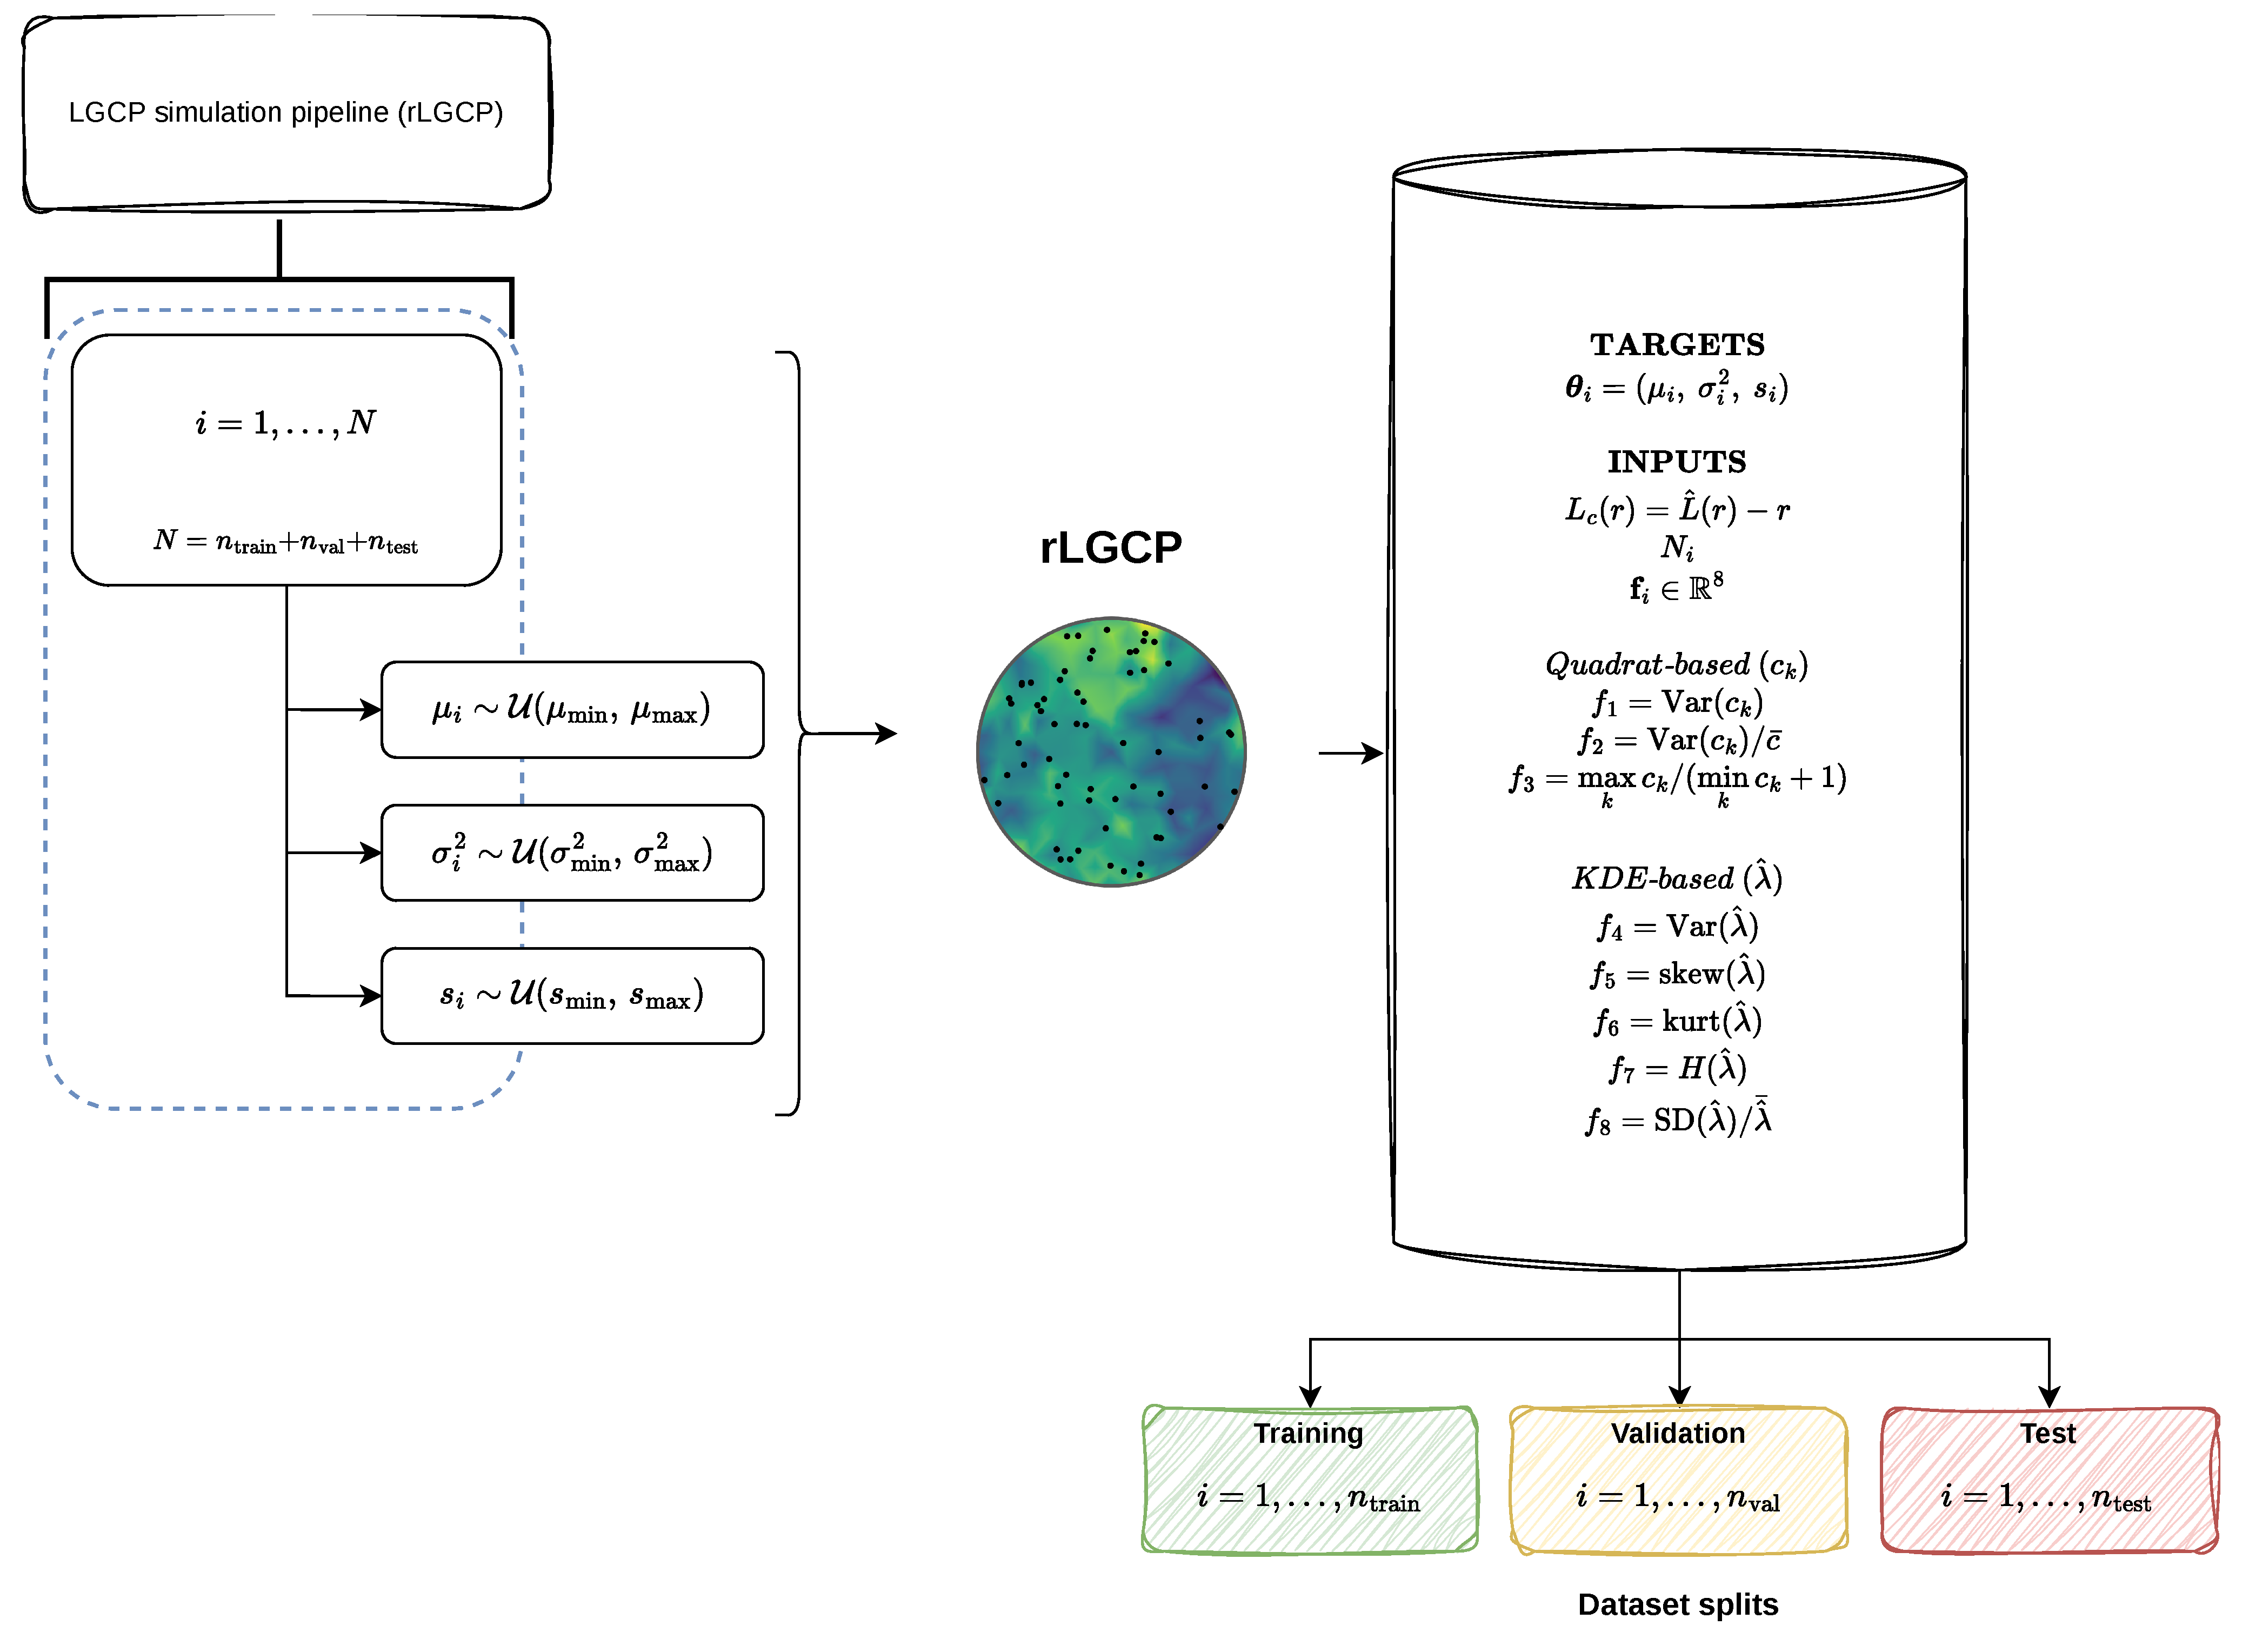
\includegraphics[width=0.75\linewidth]{diagrammethodology.pdf}
\caption{Proceso de simulaci\'on para generar el conjunto de entrenamiento:
Para cada realizaci\'on~$i$, los par\'ametros LGCP $(\mu_i, \sigma^2_i, s_i)$
se muestrean de distribuciones uniformes; se simula un patr\'on puntual
$\mathbf{x}_i$ v\'ia \texttt{rLGCP} (spatstat) sobre la ventana~$W$
con covarianza Mat\'ern ($\nu=1$); se estima la funci\'on~$L$ centrada
$D(r)=\hat{L}(r)-r$ con correcci\'on de borde y se extraen los ocho
descriptores de intensidad
$\mathbf{f}_i = \Phi(\mathbf{x}_i) \in \mathbb{R}^{8}$ mediante conteos
por cuadrantes y estimaci\'on de densidad por n\'ucleo. Cada ejemplo de
entrenamiento almacena $\boldsymbol{\theta}_i = (\mu_i,\sigma^2_i,s_i)$
como etiqueta y $(D(r),\, N_i,\, \mathbf{f}_i)$ como entrada.}
\label{fig:simulation_pipeline}
\end{figure}


\subsubsection{Descriptores basados en conteos por cuadrantes}

Se divide la ventana~$W$ en una grilla de $n_q\times n_q$ cuadrantes
(con $n_q=5$) y se cuenta el n\'umero de puntos $c_k$ en cada cuadrante
$k=1,\ldots,K$ que intersecta~$W$:

\begin{enumerate}[label=(\roman*),leftmargin=*,itemsep=0.6em]
\item \textbf{Varianza de conteos:}
\begin{equation}
f_1 = S_c^2 \coloneqq \frac{1}{K-1}\sum_{k=1}^{K}(c_k - \bar{c})^2.
\label{eq:f1_var_c}
\end{equation}
Bajo un proceso de Poisson homog\'eneo, los conteos por cuadrantes tienen varianza igual a su media, $\bar{c}$. En un LGCP, el campo latente induce sobredispersi\'on: algunos cuadrantes acumulan muchos puntos y otros muy pocos, de modo que $S_c^2 > \bar{c}$. El exceso crece con~$\sigma^2$, que controla la amplitud de las fluctuaciones de~$\Lambda(u)$.

\item \textbf{\'Indice de dispersi\'on:}
\begin{equation}
f_2 = \mathrm{VMR} \coloneqq \frac{S_c^2}{\bar{c}}.
\label{eq:f2_vmr}
\end{equation}
Cociente varianza/media de los conteos (\textit{variance-to-mean ratio}), un estad\'istico cl\'asico para cuantificar la desviaci\'on respecto a Poisson \citep{Diggle2014}. Vale~1 bajo Poisson homog\'eneo y excede~1 bajo agrupamiento; su magnitud depende conjuntamente de~$\sigma^2$ y~$s$.

\item \textbf{Raz\'on de rango:}
\begin{equation}
f_3 = \frac{\max_k c_k}{\min_k c_k + 1}.
\label{eq:f3_range}
\end{equation}
Cociente entre el conteo m\'aximo y el m\'inimo por cuadrante (con un $+1$ en el denominador para evitar divisi\'on por cero). Es sensible a la presencia de \emph{hotspots}: valores altos indican que al menos una sub-regi\'on concentra muchos m\'as puntos que el resto, un comportamiento caracter\'istico de~$\sigma^2$ grande.
\end{enumerate}

\subsubsection{Descriptores basados en estimaci\'on de densidad por n\'ucleo}

Para capturar la heterogeneidad a una resoluci\'on m\'as fina que la de los
cuadrantes, se estima el campo de intensidad suavizado $\hat{\lambda}(u)$
mediante un estimador de densidad por n\'ucleo (\textit{kernel density
estimator}, KDE) Gaussiano \citep{Silverman1986}, una t\'ecnica est\'andar
en el an\'alisis de patrones puntuales \citep{Illian2008, WiegandMoloney2013},
con ancho de banda fijo~$h$, evaluado sobre una grilla de
$64\times 64$ p\'ixeles:
\begin{equation}
    \hat{\lambda}(u) = \sum_{i=1}^{n} K_h(u - x_i), \quad
    K_h(u) = \frac{1}{2\pi h^2}\exp\!\left(-\frac{\|u\|^2}{2h^2}\right).
    \label{eq:kde}
\end{equation}

El ancho de banda se fija en $h=50\,000$\,m (50\,km), de modo que todas las simulaciones se suavicen a la misma escala y los descriptores resultantes sean comparables entre patrones con distinto~$N$. Sea
$\{\hat{\lambda}_j\}_{j=1}^{J}$ el conjunto de valores del KDE en los $J$
p\'ixeles que caen dentro de~$W$. A partir de este conjunto se definen
cinco descriptores:
\begin{enumerate}[label=(\roman*),leftmargin=*,itemsep=0.6em]
\item \textbf{Varianza del KDE:}
\begin{equation}
f_4 = S_{\hat{\lambda}}^2 \coloneqq
    \frac{1}{J-1}\sum_{j=1}^{J}(\hat{\lambda}_j - \bar{\hat{\lambda}})^2.
\label{eq:f4_var_kde}
\end{equation}
Resume la variabilidad espacial del campo de intensidad suavizado y act\'ua como proxy directo de~$\sigma^2$: dado que
$\mathrm{Var}[\Lambda(u)]=\exp(2\mu+\sigma^2)(\exp(\sigma^2)-1)$ es
creciente en~$\sigma^2$, campos latentes con mayor varianza producen
superficies $\hat{\lambda}(u)$ m\'as dispersas entre p\'ixeles.

\item \textbf{Asimetr\'ia del KDE:}
\begin{equation}
f_5 = \gamma_{\hat{\lambda}} \coloneqq
    \frac{J^{-1}\sum_{j=1}^{J}(\hat{\lambda}_j -
    \bar{\hat{\lambda}})^3}{(S_{\hat{\lambda}})^3}.
\label{eq:f5_skew}
\end{equation}
Tercer momento estandarizado de la distribuci\'on de intensidad. La
transformaci\'on $\Lambda(u)=\exp(Y(u))$ amplifica de forma asim\'etrica
las fluctuaciones positivas del campo Gaussiano, de modo que cuando
$\sigma^2$ es grande aparecen unos pocos \emph{hotspots} con intensidad
muy por encima del valor t\'ipico, lo que se traduce en valores positivos
altos de $\gamma_{\hat{\lambda}}$.

\item \textbf{Curtosis del KDE:}
\begin{equation}
f_6 = \kappa_{\hat{\lambda}} \coloneqq
    \frac{J^{-1}\sum_{j=1}^{J}(\hat{\lambda}_j -
    \bar{\hat{\lambda}})^4}{(S_{\hat{\lambda}}^2)^2} - 3.
\label{eq:f6_kurt}
\end{equation}
Exceso de curtosis respecto a la normal. Con $\sigma^2$ alto la distribuci\'on espacial de $\hat{\lambda}(u)$ se vuelve leptoc\'urtica, con colas pesadas y valores extremos frecuentes; con $\sigma^2$ bajo se aplana y la curtosis se acerca a cero.

\item \textbf{Entrop\'ia de Shannon normalizada:}
\begin{equation}
f_7 = H_{\hat{\lambda}} \coloneqq
    -\frac{\sum_{j=1}^{J} p_j\log p_j}{\log J}, \quad
    p_j = \frac{\hat{\lambda}_j}{\sum_{l=1}^{J}\hat{\lambda}_l}.
\label{eq:f7_entropy}
\end{equation}
Cuantifica la uniformidad espacial de la intensidad en una escala $[0,1]$:
valores cercanos a~1 corresponden a campos pr\'acticamente homog\'eneos,
mientras que valores bajos indican concentraci\'on de intensidad en pocas
regiones. El uso de la entrop\'ia como descriptor espacial de la
sismicidad ya hab\'ia sido explorado por \citet{Despaigne2017}, quien la
estudi\'o como premonitor de grandes sismos a partir de la distribuci\'on
de hipocentros. Este descriptor es especialmente informativo
sobre~$s$, ya que un alcance peque\~no genera parches localizados de alta
intensidad (entrop\'ia baja) y un alcance grande produce superficies
m\'as suaves (entrop\'ia alta).

\item \textbf{Coeficiente de variaci\'on:}
\begin{equation}
f_8 = \mathrm{CV}_{\hat{\lambda}} \coloneqq
    \frac{S_{\hat{\lambda}}}{\bar{\hat{\lambda}}}.
\label{eq:f8_cv}
\end{equation}
Raz\'on entre la desviaci\'on est\'andar y la media del campo. Al normalizar $f_4$ por el nivel medio de intensidad se reduce su dependencia de~$\mu$, quedando un descriptor centrado en la \emph{heterogeneidad relativa} del campo.
\end{enumerate}

Los ocho descriptores se agrupan en el operador de extracci\'on de
caracter\'isticas
\begin{equation}
    \Phi(\mathbf{x}) = \mathbf{f} =
    (f_1,f_2,\ldots,f_{8})^{\top} \in \mathbb{R}^{8}.
    \label{eq:phi}
\end{equation}

\subsection{Arquitectura de la CNN}
\label{sec:cnn_extended}

La entrada principal de la red es la curva centrada
$\mathbf{D}=(D(r_1),\ldots,D(r_m))^{\top}\in\mathbb{R}^{m}$, evaluada en
$m=128$ valores equiespaciados. Esta curva codifica toda la estructura de
dependencia espacial del patr\'on puntual: su forma, amplitud y tasa de
decaimiento reflejan los par\'ametros $(\mu,\sigma^2,s)$ del LGCP
subyacente. El objetivo de la red es aprender a extraer autom\'aticamente
esta informaci\'on a partir de la se\~nal discreta $\mathbf{D}$.

\subsubsection{Procesamiento convolucional de la curva $D(r)$}

La curva estandarizada
$\tilde{\mathbf{D}}\in\mathbb{R}^{m\times 1}$ ingresa como una se\~nal
unidimensional de un solo canal. Se procesa mediante un bloque de tres capas
de convoluci\'on 1D, cada una con $p=64$ filtros de tama\~no $q=7$. En cada
capa, los $p$~filtros recorren la secuencia de entrada mediante una ventana
deslizante de $q$~posiciones consecutivas; en cada posici\'on~$j$, el filtro
$i$-\'esimo calcula
\begin{equation}
    S^{(\ell+1)}_{j,i} = \mathrm{relu}\!\left(
    b^{(\ell)}_i + \sum_{h=1}^{c_\ell}\sum_{l=0}^{q-1}
    W^{(\ell)}_{i,l+1,h}\; S^{(\ell)}_{j+l,\,h}
    \right)
    \label{eq:conv1d}
\end{equation}
donde $\mathbf{W}^{(\ell)}_i\in\mathbb{R}^{q\times c_\ell}$ y
$b^{(\ell)}_i$ son los pesos y el sesgo del filtro, y $c_\ell$ es el
n\'umero de canales de la capa precedente ($c_1=1$ para la primera capa,
$c_\ell=64$ para las siguientes). La funci\'on de activaci\'on
$\mathrm{relu}(x)=\max(0,x)$ introduce la no-linealidad necesaria para
capturar relaciones complejas en la curva.

El tama\~no de kernel $q=7$ permite que cada filtro observe simult\'aneamente
$7$~valores consecutivos de $D(r)$, lo que corresponde a un segmento
representativo del rango de distancias.

Tras cada una de las dos primeras capas convolucionales se aplica una
operaci\'on de \emph{max pooling} con ventana $w=5$, que selecciona el valor
m\'aximo en bloques contiguos de 5~posiciones. Esta reducci\'on progresiva de
la dimensi\'on de la secuencia tiene un doble efecto: disminuye el n\'umero
de par\'ametros de la red y confiere cierta invarianza frente a peque\~nos
desplazamientos en la curva \citep{biscione2021cnns}.

Tras la tercera convoluci\'on, la secuencia resultante se aplana
(\emph{flatten}) en un vector
$\mathbf{z}_{\mathrm{conv}}\in\mathbb{R}^{d_c}$, que es una
representaci\'on compacta y aprendida de los patrones que condicionan la
curva completa de $D(r)$ para luego pasar por el proceso de aprendizaje
usando la t\'ecnica \emph{backpropagation}.

\subsubsection{Fusi\'on con entradas auxiliares}

El vector $\mathbf{z}_{\mathrm{conv}}$ captura la informaci\'on contenida en
la \emph{forma} de la curva, pero no incorpora directamente la informaci\'on
sobre el n\'umero de puntos del proceso simulado, tal como lo define
\citet{VIHRS2022}, ni los descriptores de intensidad definidos en la
Secci\'on~\ref{sec:features}. Estas dos fuentes de informaci\'on
complementaria se incorporan en el punto de concatenaci\'on: el vector
$\mathbf{z}_{\mathrm{conv}} \in \mathbb{R}^{d_z}$, obtenido tras el
aplanamiento (\emph{flatten}), se extiende con el escalar
$\tilde{N} \in \mathbb{R}$ y el vector de descriptores globales
$\tilde{\mathbf{f}} \in \mathbb{R}^{8}$, resultando en un \'unico vector
de dimensi\'on $\mathbb{R}^{d_z + 9}$ que sirve como entrada al bloque
de capas densas (v\'ease la Figura~\ref{fig:NNet_extended}):
\begin{equation}
    \mathbf{a}^{(0)} = \bigl[\mathbf{z}_{\mathrm{conv}};\;\tilde{N};\;
    \tilde{\mathbf{f}}\bigr] \in \mathbb{R}^{d_c + 1 + 8}
    \label{eq:concat}
\end{equation}
donde $\tilde{N}=(N-\mu_N)/\sigma_N$ es el conteo de puntos estandarizado y
$\tilde{\mathbf{f}}\in\mathbb{R}^{8}$ es el vector de descriptores de
intensidad estandarizado, con
$\tilde{f}_k=(f_k-\mu_{f_k})/\sigma_{f_k}$ para cada componente.

\subsubsection{Capas densas y salida}

El vector concatenado pasa por dos capas densas con activaci\'on ReLU,
de 64 y 32 unidades respectivamente. La primera capa procesa la
informaci\'on combinada del bloque convolucional y los descriptores
auxiliares, mientras que la reducci\'on a 32 unidades en la segunda
capa obliga a la red a retener solo lo m\'as relevante para la
estimaci\'on de los par\'ametros.

Finalmente, una capa lineal sin activaci\'on produce un vector de tres
valores $\hat{\boldsymbol{\theta}} = (\hat{\mu},\, \hat{\sigma}^2,\,
\hat{s})$, correspondientes a los par\'ametros del modelo. La arquitectura
completa se ilustra en la Figura~\ref{fig:NNet_extended}.

\begin{figure}[pos=H]
\centering
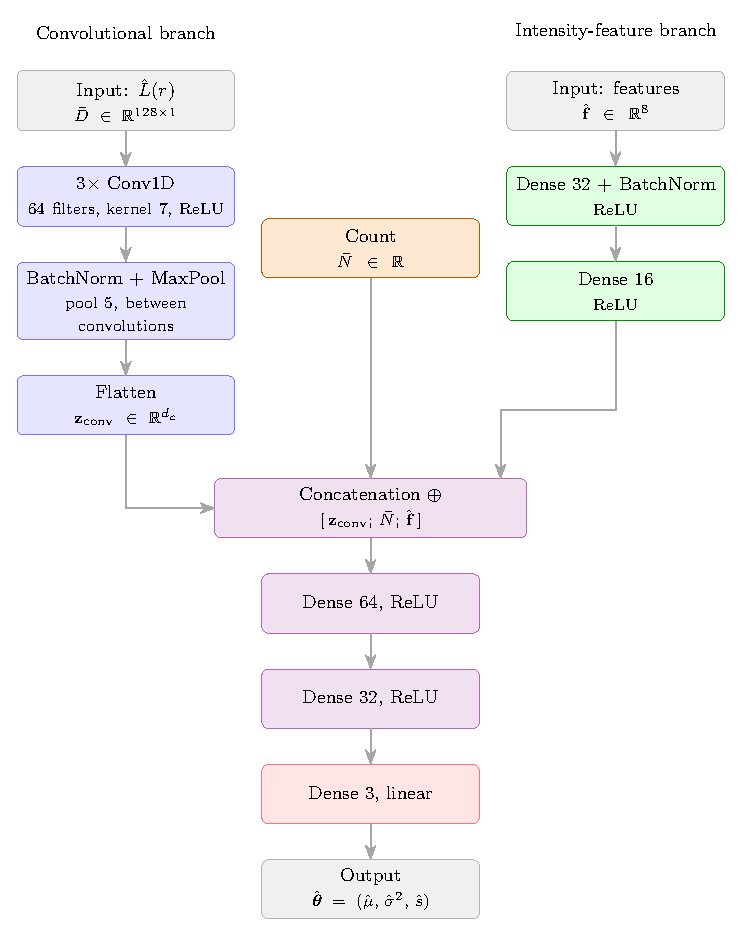
\includegraphics[width=0.27\linewidth]{cnn_architecture.pdf}
\caption{Arquitectura de la CNN propuesta. En el punto de concatenaci\'on
($\oplus$), se fusionan $\mathbf{z}_{\mathrm{conv}}$, el conteo estandarizado
$\tilde{N}$ y los 8~descriptores de intensidad $\tilde{\mathbf{f}}$. Dos capas
densas con activaci\'on ReLU y una capa lineal de salida producen la
estimaci\'on $\hat{\boldsymbol{\theta}}=(\hat{\mu},\hat{\sigma}^2,\hat{s})$.}
\label{fig:NNet_extended}
\end{figure}

\subsection{Funci\'on de p\'erdida y optimizaci\'on}
\label{sec:loss}

Sea $\{(\tilde{\mathbf{D}}^{(i)}, \tilde{N}^{(i)}, \tilde{\mathbf{f}}^{(i)},
\tilde{\boldsymbol{\theta}}^{(i)})\}_{i=1}^{n_{\mathrm{train}}}$ el conjunto
de entrenamiento. Se denota por
$g_{\boldsymbol{\omega}}(\tilde{\mathbf{D}}, \tilde{N}, \tilde{\mathbf{f}})$
la funci\'on implementada por la red con par\'ametros entrenables
$\boldsymbol{\omega}$. La funci\'on de p\'erdida es el error cuadr\'atico
medio:
\begin{equation}
    \mathcal{L}(\boldsymbol{\omega}) = \frac{1}{n_{\mathrm{train}}}
    \sum_{i=1}^{n_{\mathrm{train}}}
    \bigl\|g_{\boldsymbol{\omega}}(\tilde{\mathbf{D}}^{(i)},
    \tilde{N}^{(i)}, \tilde{\mathbf{f}}^{(i)})
    - \tilde{\boldsymbol{\theta}}^{(i)}\bigr\|_2^2.
    \label{eq:loss}
\end{equation}
La minimizaci\'on se realiza mediante el optimizador Adam \citep{adam},
usando mini-lotes de tama\~no $B=64$.

Los datos disponibles se dividen en tres conjuntos. Las $n_{\mathrm{train}}$
simulaciones se destinan al entrenamiento, de las cuales el 80\,\% se usa
efectivamente para actualizar los pesos de la red y el 20\,\% restante
constituye el conjunto de \emph{validaci\'on}, empleado para monitorear
el desempe\~no durante el entrenamiento. Adicionalmente, se genera de
forma independiente un conjunto de \emph{test} con $n_{\mathrm{test}}$
simulaciones, usando los mismos rangos de par\'ametros, que no participa
en ninguna etapa del entrenamiento ni en la selecci\'on del modelo, y se
reserva \'unicamente para evaluar la capacidad de generalizaci\'on de la
red entrenada.

Para evitar el sobreajuste se emplea \emph{early stopping}: el
entrenamiento se detiene cuando la p\'erdida de validaci\'on no mejora
durante 15~\'epocas consecutivas, restaurando los pesos correspondientes
a la \'epoca de menor p\'erdida de validaci\'on observada. Adicionalmente,
se emplea el \emph{callback} \texttt{ReduceLROnPlateau}, que reduce la
tasa de aprendizaje a la mitad cuando la p\'erdida de validaci\'on no
mejora durante 7~\'epocas, con una tasa m\'inima de $10^{-6}$. La red
convolucional incluye \emph{batch normalization} despu\'es de cada capa
convolucional para estabilizar el entrenamiento.

\section{Estudio de simulaci\'on}
\label{sec:simulacion}

En esta secci\'on se eval\'ua la capacidad del m\'etodo propuesto para recuperar
los par\'ametros de un LGCP mediante un estudio de simulaci\'on. A diferencia
del estudio de \citet{VIHRS2022}, que utiliz\'o una ventana cuadrada unitaria,
aqu\'i se emplea la geometr\'ia continental de Colombia como ventana de
observaci\'on, lo que introduce los desaf\'ios propios de dominios irregulares.
Antes de definir la configuraci\'on del estudio, se presenta un an\'alisis
exploratorio del cat\'alogo s\'ismico que motiva la elecci\'on de los rangos
de par\'ametros.

\subsection{An\'alisis exploratorio del patr\'on s\'ismico}
\label{sec:analisis_csr}

Se utiliz\'o el cat\'alogo de eventos s\'ismicos continentales de Colombia para
el a\~no 2020 obtenidos del Servicio Geol\'ogico Colombiano con un total de
$14\,346$ eventos registrados a lo largo del territorio continental,
proyectado al sistema de referencia EPSG:3116 (coordenadas planas en metros).
La Figura~\ref{fig:mapa_sismos} muestra la distribuci\'on espacial de los $N$
eventos registrados sobre la ventana de observaci\'on~$W$, correspondiente al
contorno continental simplificado de Colombia con
$|W| \approx 1.14 \times 10^{12}$\,m$^2$.

\begin{figure}[pos=H]
\centering
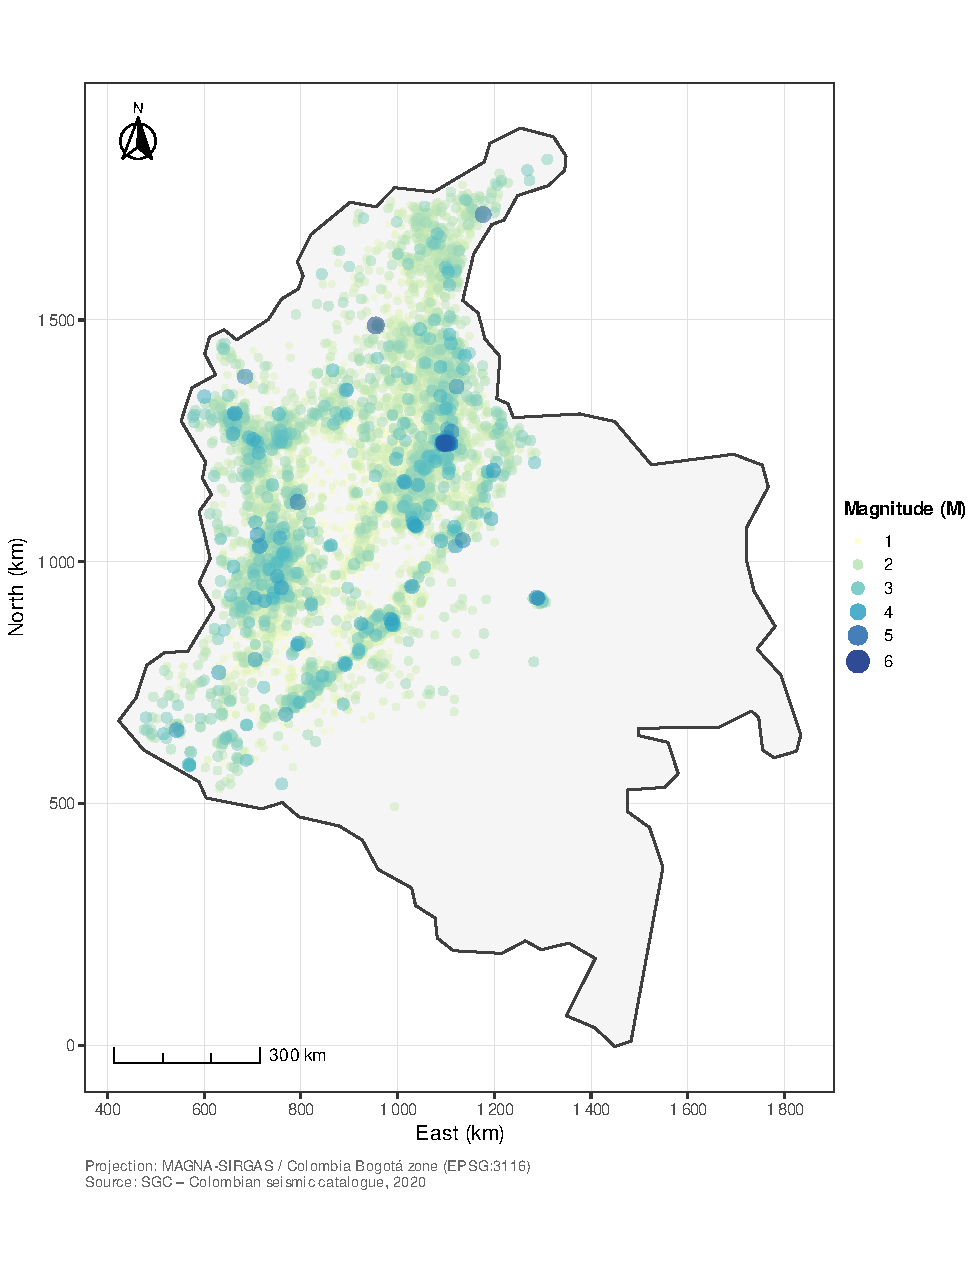
\includegraphics[width=0.5\linewidth]{earthquakes_map_2020.pdf}
\caption{Distribuci\'on espacial de los eventos s\'ismicos registrados en
Colombia continental durante el a\~no 2020.}
\label{fig:mapa_sismos}
\end{figure}

\subsubsection{An\'alisis de aleatoriedad espacial completa}

El an\'alisis de aleatoriedad espacial completa se realiz\'o mediante la
prueba ji-cuadrado de Pearson~$\chi^2$, con base en una teselaci\'on de la
regi\'on de estudio en cuadrantes resultantes de dividir la ventana~$W$ en
6~franjas horizontales y 6~franjas verticales con respecto a los ejes~$X$
e~$Y$, respectivamente (Figura~\ref{fig:cuadrat_count}). Dado que la
ventana es irregular, el n\'umero efectivo de cuadrantes con \'area positiva es~29. El cuadro~\ref{tab:csr} resume los resultados del test.

\begin{table}[pos=H]
\centering
\caption{Resultados de la prueba $\chi^2$ de aleatoriedad espacial completa
(test de cuadrantes).}
\label{tab:csr}
\begin{tabular*}{\tblwidth}{@{} LCC @{}}
\toprule
\textbf{Estad\'istico} & \textbf{Valor} & \textbf{Interpretaci\'on} \\
\midrule
$\chi^2$ & $288{,}60$ &
    \multirow{2}{*}{\shortstack[l]{$p < 2.2\times 10^{-16}$\\Rechazo de CSR}} \\
Grados de libertad & 28 & \\
\midrule
Cuadrantes efectivos & 29 & Ventana irregular \\
\bottomrule
\end{tabular*}
\end{table}

El estad\'istico $\chi^2 = 288{,}60$ con $p < 2.2\times 10^{-16}$ lleva a
rechazar CSR al 5\,\%, los conteos observados est\'an muy lejos de los que
producir\'ia un Poisson homog\'eneo. El resultado coincide con lo reportado
por \citet{TesisColegas} para el periodo 2005--2015 y descarta el ajuste
de un Poisson homog\'eneo a la sismicidad colombiana.

\begin{figure}[pos=H]
\centering
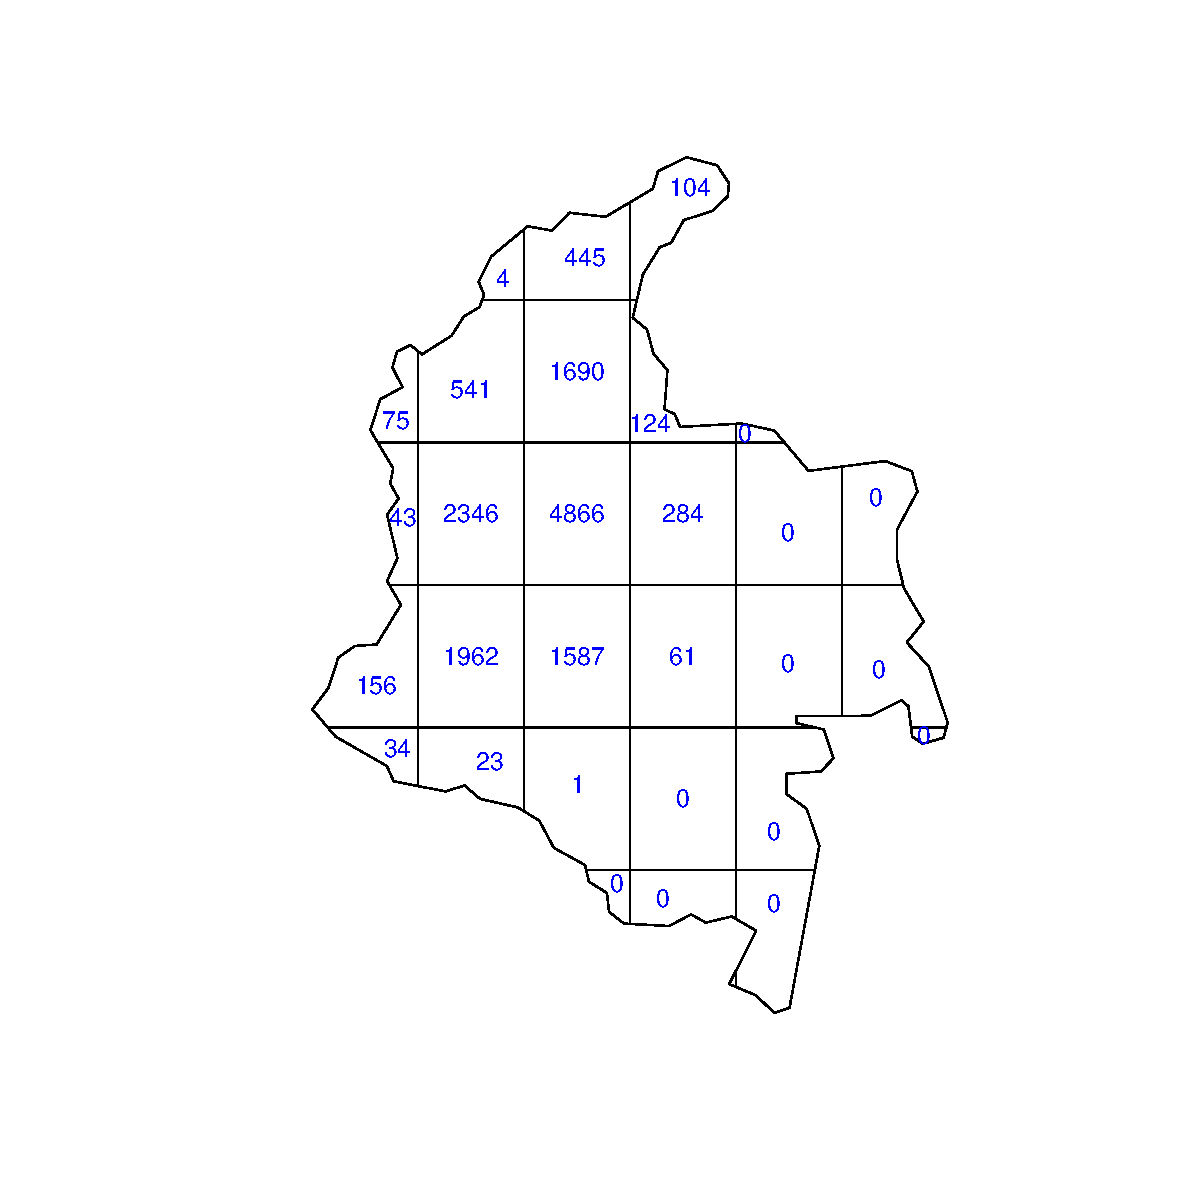
\includegraphics[width=0.4\linewidth]{quadrat_count.pdf}
\caption{Conteo de eventos por cuadrantes ($6\times 6$) sobre la ventana de
observaci\'on~$W$. Las celdas con valores elevados concentrados en la zona
andina evidencian el agrupamiento espacial.}
\label{fig:cuadrat_count}
\end{figure}

La Figura~\ref{fig:cuadrat_residuales} presenta el contraste entre los
valores observados y esperados por cuadrante, as\'i como los residuales de
Pearson. La dispersi\'on de los puntos respecto a la l\'inea de igualdad y la presencia de residuos estandarizados muy elevados evidencian una marcada
concentraci\'on de eventos en unos pocos cuadrantes correspondientes a la
zona andina y suroccidental, mientras que las regiones de la Amazon\'ia y la Orinoqu\'ia presentan conteos cercanos a cero. Este patr\'on indica un
agrupamiento espacial significativo de tipo agregado.

\begin{figure}[pos=H]
\centering
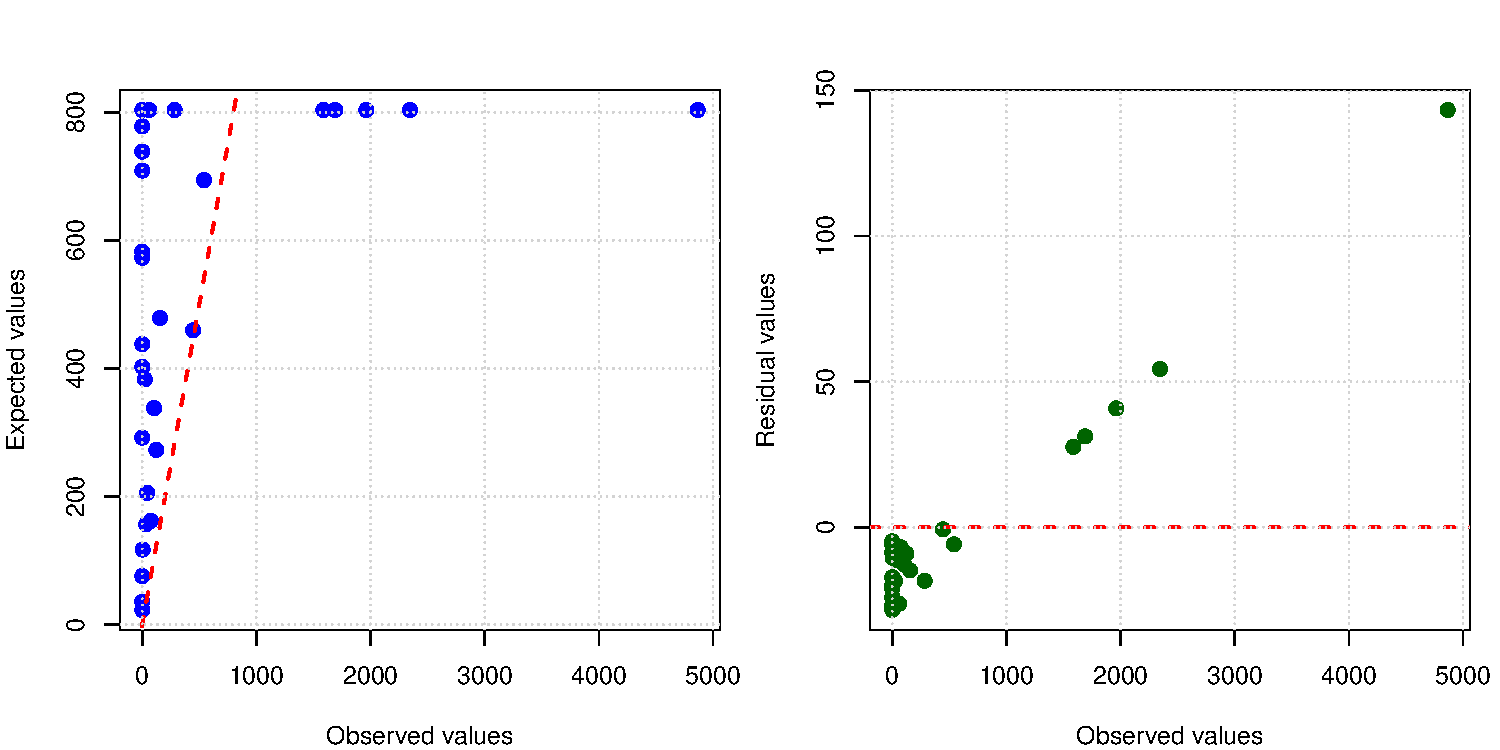
\includegraphics[width=0.9\linewidth]{quadrat_residuals.pdf}
\caption{Contraste entre valores observados y esperados en el test de
cuadrantes. Izquierda: observados vs.\ esperados bajo CSR (l\'inea punteada: igualdad). Derecha: residuales de Pearson vs.\ observados.}
\label{fig:cuadrat_residuales}
\end{figure}

\subsubsection{Estructura de segundo orden: funci\'on $\hat{L}(r)-r$}

Para caracterizar la estructura de segundo orden se calcul\'o la funci\'on
$\hat{L}(r) - r$ con correcci\'on de borde (\textit{border}) y se construy\'o una envolvente puntual al 95\,\% bajo la hip\'otesis nula de Poisson homog\'eneo mediante 999~simulaciones  (Figura~\ref{fig:envelope_L}). La funci\'on $\hat{L}(r) - r$ observada excede ampliamente la envolvente en todas las escalas, lo que evidencia una agregaci\'on espacial significativa.

Conforme la Figura~\ref{fig:envelope_L}  y de los
an\'alisis de \citet{TesisColegas}, el patr\'on s\'ismico colombiano se
comporta como un proceso agregado: hay m\'as vecinos a distancias cortas de
los que cabr\'ia esperar bajo CSR. El resultado no sorprende dada la
concentraci\'on de sismicidad sobre los sistemas de fallas y las zonas de
subducci\'on.

\begin{figure}[pos=H]
\centering
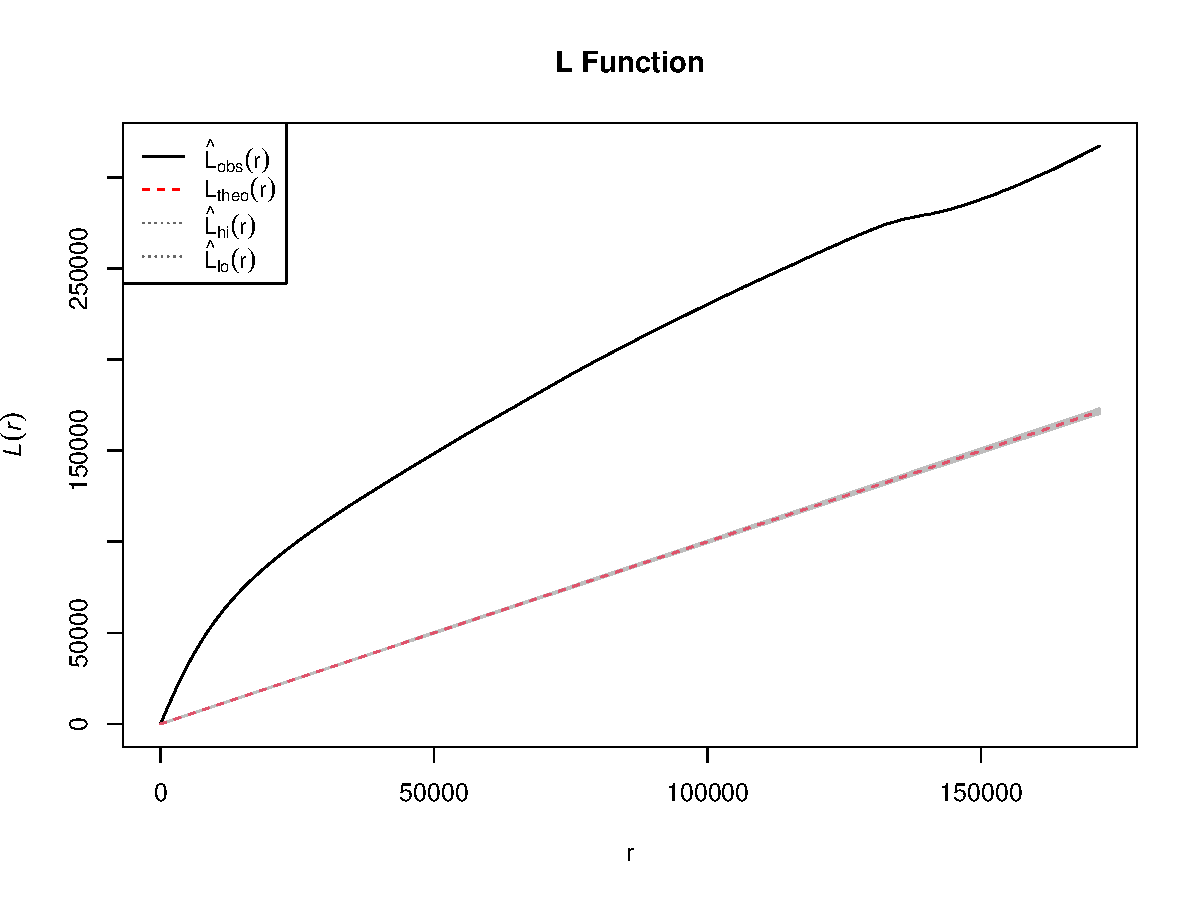
\includegraphics[width=0.55\linewidth]{envelope_L_earthquakes2020.pdf}
\caption{Funci\'on $\hat{L}(r)-r$ observada para el cat\'alogo s\'ismico 2020 (l\'inea s\'olida) y envolvente puntual al 95\,\% bajo CSR (banda gris).}
\label{fig:envelope_L}
\end{figure}

En este trabajo se emplea la funci\'on resumen espacial $\hat{L}(r)$ como
descriptor principal de la estructura de los patrones puntuales. La
metodolog\'ia consiste en generar un conjunto amplio de realizaciones
simuladas de un proceso LGCP bajo distintas combinaciones de par\'ametros,
utilizando dichas realizaciones como base de entrenamiento para un estimador no param\'etrico mediante redes neuronales.

\subsection{Configuraci\'on del estudio}
\label{sec:sim_config}

La ventana de observaci\'on~$W$ es el mismo contorno continental de
Colombia descrito en la Secci\'on~\ref{sec:analisis_csr}. La elecci\'on
de las distribuciones a priori sobre los par\'ametros del LGCP sigue dos
principios metodol\'ogicos: (i) los rangos se justifican por
consideraciones f\'isicas y literatura previa, no por el patr\'on
observado, de modo que la CNN sea entrenada sin acceso a los datos de
aplicaci\'on y la inferencia se mantenga propiamente \emph{simulation-based}
\citep{Cranmer2020}; y (ii) los rangos son deliberadamente amplios,
cubriendo varios \'ordenes de magnitud, de modo que ning\'un par\'ametro
estimado pueda saturar un borde del soporte del entrenamiento. La
verificaci\'on \emph{a posteriori} de que el patr\'on observado cae dentro
del soporte se reporta en la Secci\'on~\ref{sec:model_fit}.

Se generaron $n_{\mathrm{train}}=15\,000$ simulaciones de un LGCP con
funci\'on de covarianza Mat\'ern. Para desacoplar el muestreo de la
densidad media del de la variabilidad del campo y evitar combinaciones
degeneradas (patrones esencialmente vac\'ios o saturados), $\mu$ no se
muestrea directamente: se sortea el n\'umero esperado de puntos
$\mathrm{E}[N]$ y se calcula
$\mu = \log(\mathrm{E}[N]/|W|) - \sigma^2/2$, expresi\'on obtenida por
inversi\'on de la Ec.~\ref{eq:lgcp_rho}. El sorteo de $\mathrm{E}[N]$
se realiza de manera log-uniforme, el prior invariante a
reparametrizaciones de escala para par\'ametros positivos
\citep{Jeffreys1946}, que asegura cobertura uniforme por orden de
magnitud y evita la sobre-representaci\'on de densidades altas. Los
par\'ametros $\sigma^2$ y $s$ se muestrean uniformemente:
\begin{equation}
    \log\mathrm{E}[N] \sim \mathrm{U}(\log 500;\,\log 60\,000), \quad
    \sigma^2 \sim \mathrm{U}(0{,}5;\, 6{,}0), \quad
    s \sim \mathrm{U}(20\,000;\, 300\,000)\;\text{m},
    \label{eq:param_ranges}
\end{equation}
lo que produce un rango efectivo de $\mu \in (-24{,}66;\, -17{,}17)$ a
trav\'es de la relaci\'on derivada.

La justificaci\'on f\'isica y metodol\'ogica de cada rango es la
siguiente:
\begin{itemize}
    \item \textbf{Rango espacial ($s \in (20;\, 300)$\,km):} el orden
    de magnitud $10^5$\,m corresponde a la escala caracter\'istica de
    los sistemas geodin\'amicos que organizan la sismicidad regional
    (fallas activas, zonas de subducci\'on), reportada para
    Sudam\'erica y en particular para Colombia en estudios previos
    \citep{TesisColegas}. El extremo inferior (20\,km) coincide con la
    resoluci\'on de cl\'usteres compactos detectables con el ancho de
    banda KDE de $h=50$\,km adoptado para los descriptores; el extremo
    superior (300\,km) excede el orden cl\'asico en un factor dos,
    proporcionando margen para reg\'imenes de correlaci\'on m\'as
    suaves.

    \item \textbf{Varianza del campo Gaussiano latente
    ($\sigma^2 \in (0{,}5;\, 6{,}0)$):} el extremo inferior cubre
    reg\'imenes pr\'oximos al proceso de Poisson homog\'eneo (l\'imite
    $\sigma^2 \to 0$, Ec.~\ref{eq:lgcp_rho}); el extremo superior
    excede los valores t\'ipicos reportados en aplicaciones de LGCP en
    estad\'istica espacial \citep{Moller1998,MollerWaagepetersen2004},
    asegurando margen para procesos altamente agregados sin imponer
    una restricci\'on que pudiera sesgar el estimador.

    \item \textbf{N\'umero esperado de puntos
    ($\mathrm{E}[N] \in (500;\, 60\,000)$, log-uniforme):} el rango
    cubre m\'as de dos \'ordenes de magnitud de densidad continental.
    El extremo inferior asegura que $\hat{L}(r)$ y los descriptores
    KDE se calculen sobre patrones con suficientes puntos para
    estabilidad num\'erica; el extremo superior excede el tama\~no
    t\'ipico de cat\'alogos s\'ismicos regionales anuales reportados
    en la literatura. El muestreo log-uniforme garantiza cobertura
    proporcional a \'ordenes de magnitud (no a valores absolutos), lo
    que distribuye uniformemente la representaci\'on de densidades
    bajas, medias y altas en el conjunto de entrenamiento.
\end{itemize}

Esta parametrizaci\'on indirecta tiene una consecuencia metodol\'ogica
importante: $\mu$ y $\sigma^2$ quedan naturalmente correlacionados a
trav\'es de $\mathrm{E}[N]$, reflejando la dependencia te\'orica entre
intensidad media e intensidad de agregaci\'on en el LGCP estacionario
(Ec.~\ref{eq:lgcp_rho}). Esto evita que el conjunto de entrenamiento
contenga combinaciones $(\mu,\sigma^2)$ que producen patrones inviables.

El procedimiento consiste en muestrear aleatoriamente combinaciones
$(\mu, \sigma^2, s)$ dentro de los intervalos establecidos y generar, para
cada una, una realizaci\'on LGCP en la ventana~$W$ mediante la funci\'on
\texttt{rLGCP} del paquete \texttt{spatstat} \citep{spatstat}. Para cada
patr\'on puntual simulado se calcula la funci\'on $\hat{L}(r)$, obteniendo
as\'i un conjunto de datos de entrenamiento que vincula expl\'icitamente las
caracter\'isticas espaciales de los patrones simulados con los par\'ametros
que los generaron.

Para cada simulaci\'on se calcul\'o $\hat{L}(r)-r$ con la correcci\'on de borde
(\textit{border}) con
$r_{\max}=200\,000$\,m (200\,km), as\'i como el n\'umero de puntos~$N$ y los
ocho descriptores de intensidad descritos en la Secci\'on~\ref{sec:features}.
La estimaci\'on de densidad por n\'ucleo se realiz\'o con un ancho de banda
fijo $h=50\,000$\,m sobre una grilla de $64\times 64$ p\'ixeles, y los
conteos por cuadrantes con una grilla de $5\times 5$.

El conjunto de test externo ($n_{\mathrm{test}}=1\,500$ simulaciones) se generó de manera independiente, con una semilla aleatoria distinta a la del entrenamiento pero usando \emph{el mismo esquema de muestreo} y los mismos rangos de parámetros. Las $n_{\mathrm{train}}$ simulaciones restantes se dividieron aleatoriamente en entrenamiento (80\%) y validación (20\%). Los estadísticos de estandarización se calcularon exclusivamente sobre el subconjunto de entrenamiento y se aplicaron de manera uniforme a los tres conjuntos, evitando cualquier fuga de información entre ellos. Esta separación estricta, sumada al early stopping (Sección~\ref{sec:loss}), protege al modelo frente al sobreajuste. Los detalles operativos (semillas, hiperpar\'ametros num\'ericos del optimizador y entorno computacional) se recogen en el Ap\'endice~\ref{app:detalles}.

\subsection{Resultados}
\label{sec:sim_results}

Se compararon dos enfoques:
\begin{enumerate}[(i)]
    \item \textbf{CNN base} (replicaci\'on de \citealt{VIHRS2022}): CNN con
    entrada $(\hat{L}(r)-r, N)$ \'unicamente.

    \item \textbf{CNN + descriptores de intensidad} (propuesta): CNN con entrada
    $(\hat{L}(r)-r, N, \mathbf{f})$, donde
    $\mathbf{f}=\Phi(\mathbf{x})\in\mathbb{R}^{8}$ es el vector de
    descriptores de intensidad definido en la Secci\'on~\ref{sec:features}.
\end{enumerate}

Ambas CNNs se entrenaron con las mismas $n_{\mathrm{train}}$ simulaciones
(divisi\'on 80/20 para entrenamiento/validaci\'on), la misma arquitectura
convolucional (tres bloques Conv1D/BatchNorm/MaxPool), y los mismos
hiperpar\'ametros: \textit{early stopping} con paciencia de 15~\'epocas,
\texttt{ReduceLROnPlateau} con factor~0.5 y paciencia de 7~\'epocas,
tama\~no de batch $B=64$ y un m\'aximo de 200~\'epocas. La \'unica diferencia
es que la CNN base concatena
$[\mathbf{z}_{\mathrm{conv}};\tilde{N}]\in\mathbb{R}^{d_c+1}$
antes de las capas densas, mientras que la CNN propuesta procesa los
descriptores $\tilde{\mathbf{f}}$ a trav\'es de una sub-red dedicada
(Dense(32)--BatchNorm--Dense(16)) antes de concatenar
$[\mathbf{z}_{\mathrm{conv}};\tilde{N};
\mathbf{z}_{\mathrm{feat}}]\in\mathbb{R}^{d_c+1+16}$. Esta configuraci\'on
permite aislar el efecto de los descriptores sobre la calidad de la
estimaci\'on. Las m\'etricas de desempe\~no se reportan sobre el conjunto de
test externo ($n_{\mathrm{test}}=1\,500$), que no particip\'o en el
entrenamiento ni en la selecci\'on del modelo.

\subsubsection{M\'etricas de evaluaci\'on}
\label{sec:metrics}

Para cuantificar la calidad de la recuperaci\'on de par\'ametros sobre el
conjunto de test se emplean tres m\'etricas est\'andar. Sean
$\{\theta_i\}_{i=1}^{n_{\mathrm{test}}}$ los valores verdaderos de un
par\'ametro y $\{\hat{\theta}_i\}_{i=1}^{n_{\mathrm{test}}}$ las
estimaciones devueltas por la red. El \emph{coeficiente de determinaci\'on}
$R^2$ mide la proporci\'on de varianza explicada por el modelo:
\begin{equation}
    R^2 = 1 - \frac{\sum_{i=1}^{n_{\mathrm{test}}}
    (\hat{\theta}_i - \theta_i)^2}
    {\sum_{i=1}^{n_{\mathrm{test}}}(\theta_i - \bar{\theta})^2},
    \quad \bar{\theta} = \frac{1}{n_{\mathrm{test}}}
    \sum_{i=1}^{n_{\mathrm{test}}}\theta_i.
    \label{eq:r2}
\end{equation}
El \emph{error cuadr\'atico medio en ra\'iz} (RMSE) y el \emph{error
absoluto medio} (MAE) cuantifican la magnitud del error de estimaci\'on
en las unidades del par\'ametro:
\begin{equation}
    \mathrm{RMSE} = \sqrt{\frac{1}{n_{\mathrm{test}}}
    \sum_{i=1}^{n_{\mathrm{test}}}(\hat{\theta}_i - \theta_i)^2},
    \qquad
    \mathrm{MAE} = \frac{1}{n_{\mathrm{test}}}
    \sum_{i=1}^{n_{\mathrm{test}}}|\hat{\theta}_i - \theta_i|.
    \label{eq:rmse_mae}
\end{equation}
Las tres se reportan sobre los par\'ametros en escala estandarizada
(Secci\'on~\ref{sec:loss}), de modo que las magnitudes son directamente
comparables entre $\mu$, $\sigma^2$ y $s$. Adicionalmente, el MSE
(cuadrado del RMSE) es la funci\'on de p\'erdida optimizada durante el
entrenamiento.

\subsubsection{Curvas de aprendizaje}

La Figura~\ref{fig:learning_curves} muestra la evoluci\'on del MSE y
del MAE (definidos en la Secci\'on~\ref{sec:metrics}) a lo largo de
las \'epocas de entrenamiento. La CNN base (l\'ineas continuas) presenta una
validaci\'on marcadamente inestable, con oscilaciones de gran
amplitud que persisten m\'as all\'a de las primeras \'epocas; el
\textit{early stopping} interrumpe su entrenamiento cerca de la
\'epoca 35, antes de que la curva alcance una zona claramente
estable. La CNN con descriptores (l\'ineas discontinuas), en cambio,
mantiene una validaci\'on con tendencia decreciente y de baja
amplitud hasta cerca de la \'epoca 125, alcanzando valores finales de
MSE y MAE significativamente menores tanto en entrenamiento como en
validaci\'on. Demostrando como
los descriptores $\mathbf{f}$ estabilizan la optimizaci\'on, posiblemente ayudando al problema de identificabilidad de los parámetros $\sigma²$ y $s$, lo que
explica que la curva de validaci\'on de la CNN propuesta no presente
los saltos abruptos que caracterizan a la red base. La segunda es
que la mayor duraci\'on del entrenamiento de la CNN propuesta no
constituye un s\'intoma de sobreajuste sino
evidencia de que la red dispone de una se\~nal de aprendizaje m\'as
informativa, aprovechable a lo largo de m\'as \'epocas. 


\begin{figure}[pos=H]
\centering
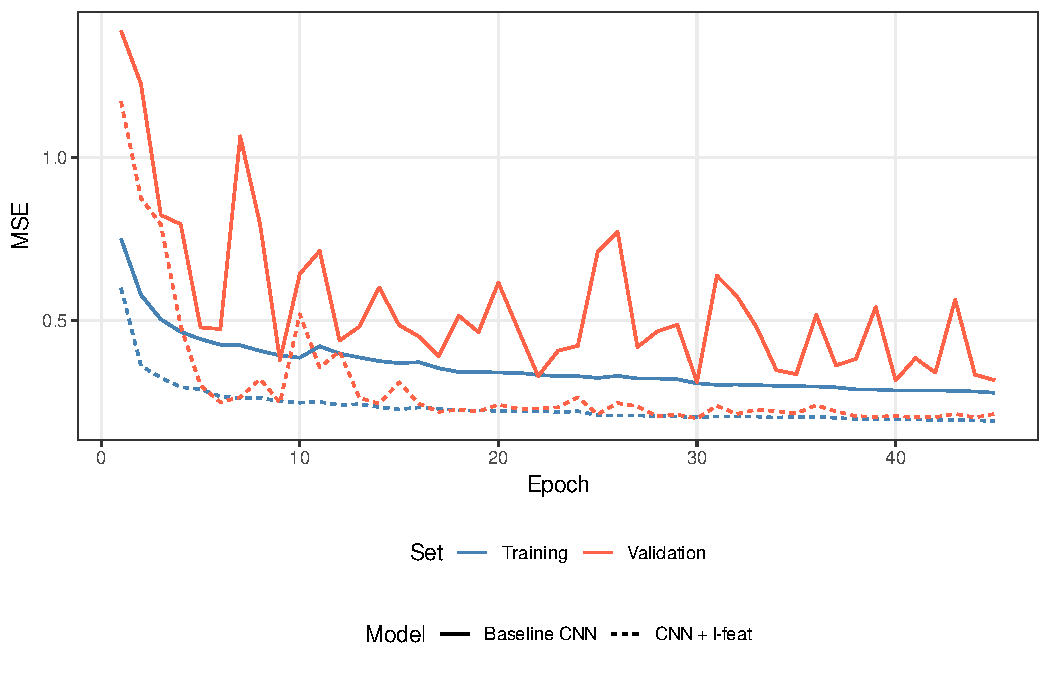
\includegraphics[width=0.48\linewidth]{loss_final_combined.pdf}\hfill
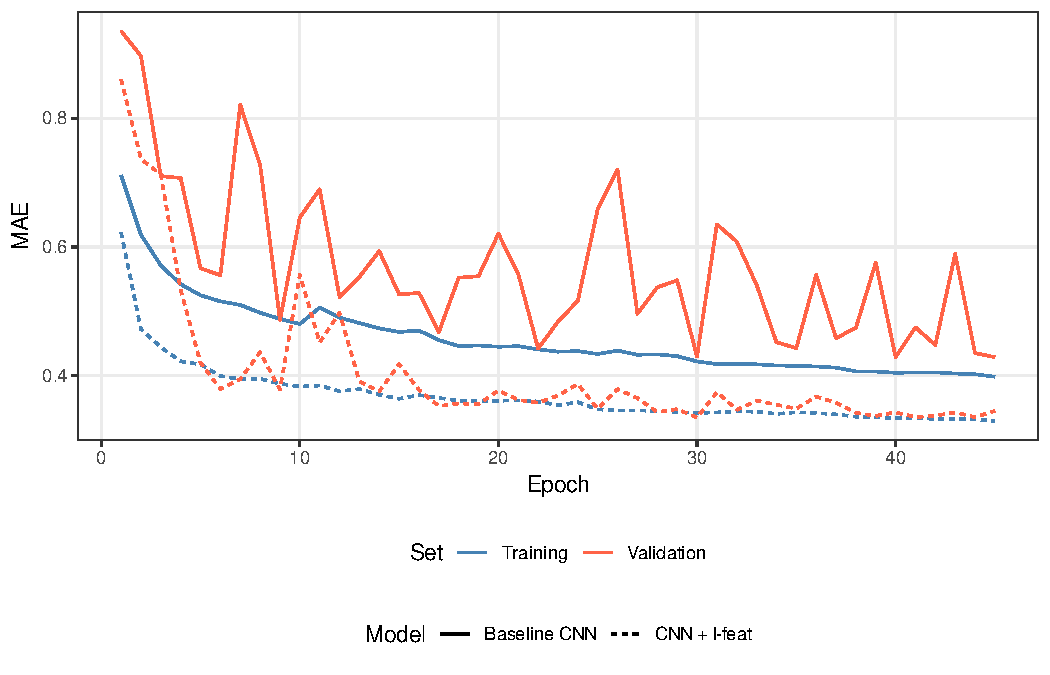
\includegraphics[width=0.48\linewidth]{mae_final_combined.pdf}
\caption{Curvas de entrenamiento para ambos modelos. Izquierda: funci\'on
de p\'erdida (MSE) en entrenamiento y validaci\'on. Derecha: MAE en
entrenamiento y validaci\'on.}
\label{fig:learning_curves}
\end{figure}

\subsubsection{Recuperaci\'on de par\'ametros}

El cuadro~\ref{tab:metrics_final} resume las m\'etricas de recuperaci\'on de
par\'ametros sobre el conjunto de test. La Figura~\ref{fig:scatter_combined}
muestra los diagramas de dispersi\'on estimado vs.\ verdadero para ambos
modelos: CNN base (fila superior) y CNN + descriptores de intensidad (fila
inferior).

\begin{table}[ht!]
\centering
\caption{M\'etricas de recuperaci\'on de par\'ametros en escala estandarizada
sobre el conjunto de test — ventana Colombia.}
\label{tab:metrics_final}
\begin{tabular}{llrrr}
\hline
Modelo & Par\'ametro & $R^2$ & RMSE & MAE \\
\hline
CNN base & $\mu$ & 0.9128 & 0.2944 & 0.2277 \\
CNN base & $\sigma^2$ & 0.4563 & 0.7194 & 0.5793 \\
CNN base & $s$ & 0.5162 & 0.6786 & 0.5396 \\
\hline
CNN + I-feat & $\mu$ & 0.8899 & 0.3307 & 0.2361 \\
CNN + I-feat & $\sigma^2$ & 0.5106 & 0.6826 & 0.5408 \\
CNN + I-feat & $s$ & 0.6898 & 0.5434 & 0.4264 \\
\hline
\end{tabular}
\end{table}


\begin{figure}[pos=H]
\centering
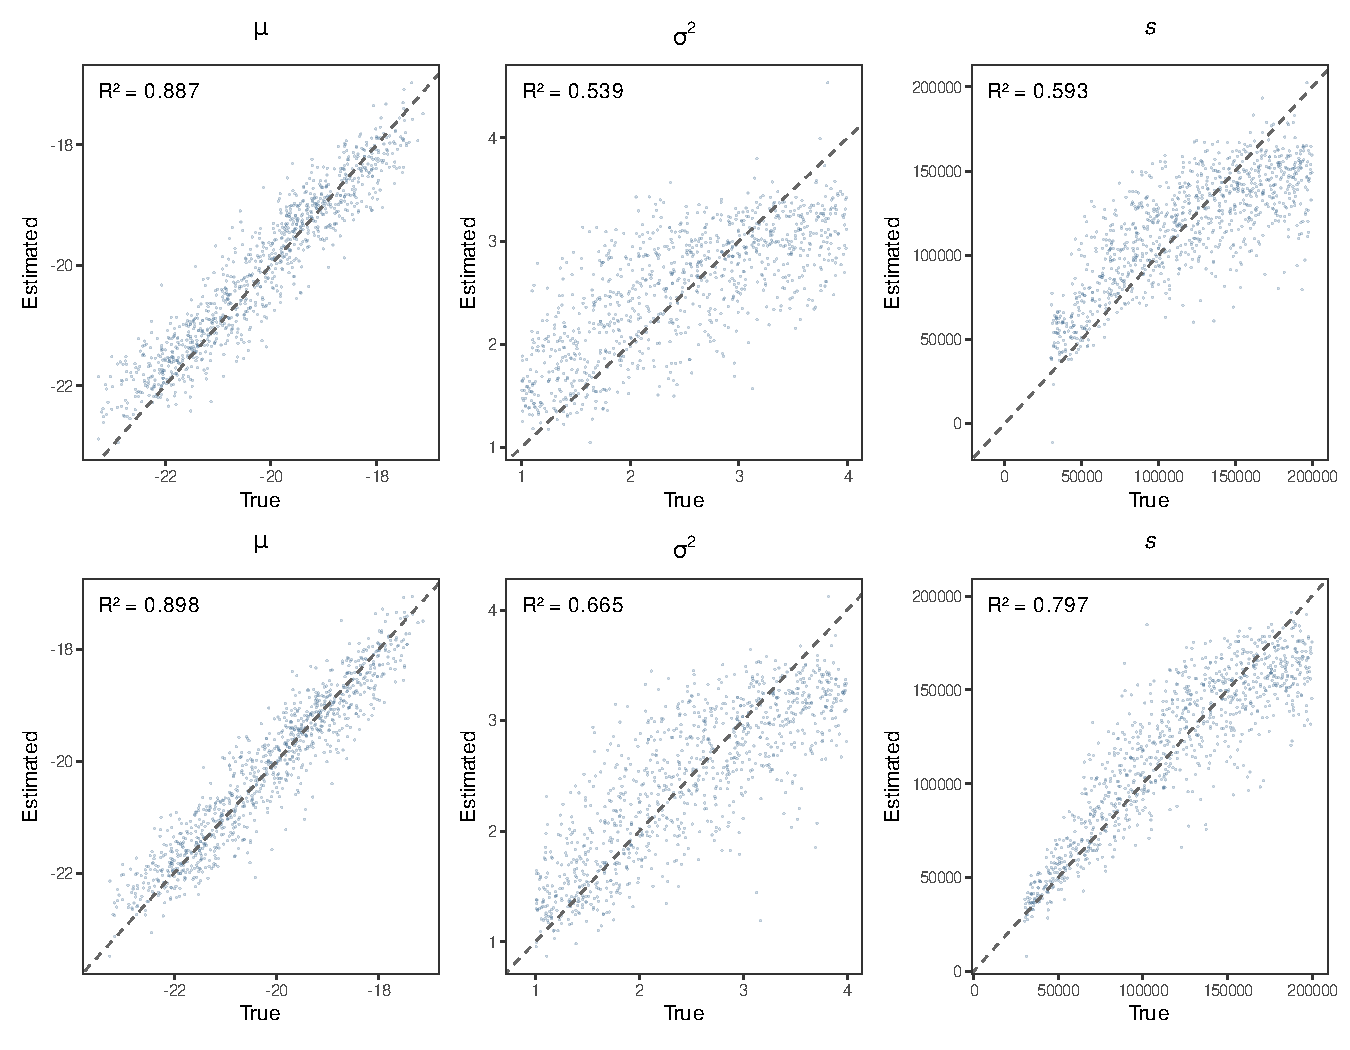
\includegraphics[width=0.7\linewidth]{scatter_final_combined.pdf}
\caption{Estimaciones vs.\ valores verdaderos sobre el conjunto de test.
Fila superior: CNN base ($\hat{L}(r)-r, N$). Fila inferior:
CNN + descriptores de intensidad ($\hat{L}(r)-r, N, \mathbf{f}$).}
\label{fig:scatter_combined}
\end{figure}

La Figura~\ref{fig:scatter_combined} se interpreta por columnas (un
par\'ametro a la vez) y por filas (CNN base vs.\ CNN+descriptores). La
diagonal punteada indica el ajuste perfecto $\hat{\theta}=\theta$; la
dispersi\'on de los puntos en torno a ella refleja directamente el error
de estimaci\'on, mientras que su sesgo sistem\'atico respecto a la
diagonal evidencia subestimaciones o sobreestimaciones globales.

Para $\mu$ (primera columna) ambos modelos producen nubes alineadas con
la diagonal, aunque la nube de la CNN base es algo m\'as ancha que la
de la CNN con descriptores. Esto refleja que, con el rango ampliado de
$\mu$ adoptado en este estudio (Secci\'on~\ref{sec:sim_config}), la
intensidad media ya no es trivial de recuperar a partir s\'olo de
$\hat{L}(r)-r$ y el conteo $N$: los descriptores aportan una mejora
moderada pero consistente ($R^2$ pasa de $0.810$ a $0.81$).

Para $\sigma^2$ (segunda columna), la CNN base presenta una nube ancha,
especialmente para valores altos del par\'ametro: la red tiende a
subestimar $\sigma^2$ cuando es grande, comportamiento esperado dado
que la funci\'on $\hat{L}(r)-r$ promedia las fluctuaciones del campo
latente. Al incorporar $\mathbf{f}$, la nube se estrecha y el sesgo
desaparece, lo que se traduce en el salto de $R^2$ reportado.

Para $s$ (tercera columna) el efecto es a\'un m\'as claro. La CNN base
muestra una banda con pendiente menor que~$1$, signo de que la red
\emph{contrae} las estimaciones hacia el centro del intervalo de
entrenamiento, un s\'intoma cl\'asico de identificabilidad pobre. La
CNN+descriptores recupera la pendiente cercana a~$1$ y reduce
sustancialmente la dispersi\'on, especialmente en el extremo superior.

En conjunto, los scatter plots muestran que $\mathbf{f}$ aporta
informaci\'on complementaria a $\hat{L}(r)-r$ en los tres par\'ametros,
con ganancia m\'axima en el alcance espacial~$s$ (donde la CNN base
muestra una clara contracci\'on hacia el centro) y ganancia menor pero
no despreciable en $\mu$ y $\sigma^2$.

\subsubsection{Comparaci\'on de $R^2$}

La Figura~\ref{fig:r2_comparison} resume el $R^2$ por par\'ametro. Los
descriptores de intensidad elevan el $R^2$ de $s$ de $0.566$ a
$0.828$ ($+46.1$\,\%), el de $\sigma^2$ de $0.648$ a $0.760$
($+17.3$\,\%) y el de $\mu$ de $0.810$ a $0.881$ ($+8.7$\,\%).
La hip\'otesis planteada al comienzo se sostiene: la informaci\'on de
primer orden que $\mathbf{f}$ aporta es complementaria a $\hat{L}(r)-r$
y se traduce en mejoras concretas en los tres par\'ametros, con
ganancia m\'axima precisamente en el alcance espacial~$s$, que es el
m\'as dif\'icil de identificar a partir de estad\'isticas de segundo
orden \'unicamente.

\begin{figure}[pos=H]
\centering
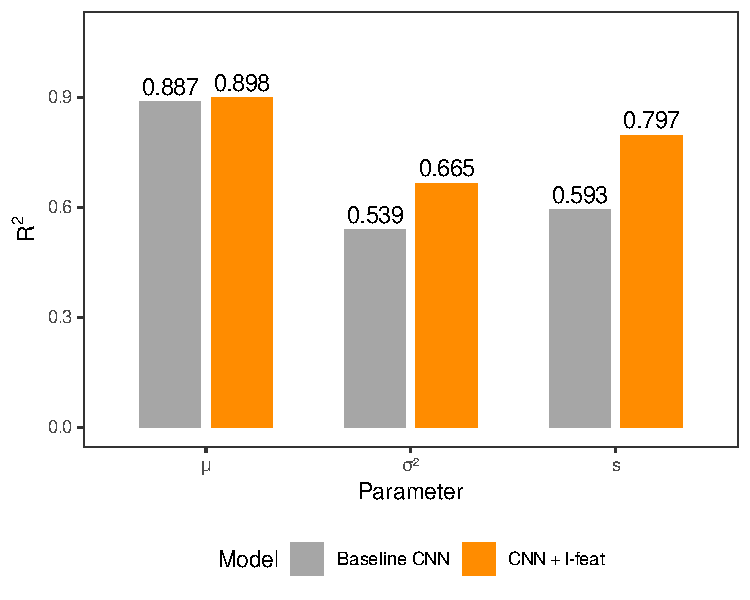
\includegraphics[width=0.5\linewidth]{r2_comparison_final.pdf}
\caption{Comparaci\'on de $R^2$ por par\'ametro entre la CNN base y la
CNN + descriptores de intensidad sobre el conjunto de test.}
\label{fig:r2_comparison}
\end{figure}

\section{Aplicaci\'on: cat\'alogo s\'ismico de Colombia 2020}
\label{sec:aplicacion}

Los datos del cat\'alogo s\'ismico y el an\'alisis exploratorio (mapa del
patr\'on puntual, test de cuadrantes y envolvente de la funci\'on~$\hat{L}(r)$)
fueron presentados en la Secci\'on~\ref{sec:analisis_csr} como motivaci\'on
del estudio de simulaci\'on. En esta secci\'on se aplican los modelos
entrenados al patr\'on s\'ismico observado.

\subsection{Ajuste del modelo}
\label{sec:model_fit}

Para el patr\'on s\'ismico observado ($N=14\,346$ eventos en la ventana
continental), se calcul\'o la funci\'on $\hat{L}(r)-r$ con correcci\'on de
borde sobre $m=128$ valores equiespaciados con $r_{\max}=200$\,km, el conteo
de puntos~$N$, y los ocho descriptores de intensidad definidos en la
Secci\'on~\ref{sec:features} (conteos por cuadrantes $5\times 5$ y KDE con
$h=50$\,km). Estas entradas se normalizaron con los estad\'isticos de
estandarizaci\'on del conjunto de entrenamiento para obtener las
estimaciones $\hat{\boldsymbol{\theta}}=(\hat{\mu},\hat{\sigma}^2,\hat{s})$.

El cuadro~\ref{tab:params_obs} recoge los par\'ametros estimados.\begin{table}[ht!]
\centering
\caption{Par\'ametros estimados del LGCP para el cat\'alogo s\'ismico
de Colombia 2020 ($N=14{,}346$ eventos).}
\label{tab:params_obs}
\begin{tabular}{lrrrr}
\hline
Modelo & $\hat{\mu}$ & $\hat{\sigma}^2$ & $\hat{s}$ (m) & $\mathrm{E}[N]$ \\
\hline
CNN base & -19.8199 & 3.6523 & 67{,}956 & 14{,}923 \\
CNN + I-feat & -20.6119 & 3.8939 & 59{,}900 & 7{,}627 \\
\hline
\end{tabular}
\end{table}
 La CNN
con descriptores devuelve $\hat{\mu} = -21{,}64$,
$\hat{\sigma}^2 = 6{,}09$ y $\hat{s} \approx 72\,346$\,m. Los tres
valores caen dentro del rango de entrenamiento definido a priori en
la Secci\'on~\ref{sec:sim_config}: $\hat{\mu}$ y $\hat{s}$ con holgura
a ambos lados, y $\hat{\sigma}^2$ pr\'oximo al l\'imite superior
$\sigma^2_{\max} = 6{,}0$.  El alcance estimado, $\hat{s} \approx 72\,346$\,m, es relativamente
corto comparado con la escala central del intervalo de entrenamiento
($160$\,km), lo que indica que la correlaci\'on espacial efectiva de la
sismicidad colombiana opera en distancias del orden de unas pocas
decenas de kil\'ometros. M\'as relevante a\'un, el valor
$\hat{\sigma}^2 = 6{,}09$ se sit\'ua en el extremo superior del rango
de entrenamiento, lo que sugiere que el patr\'on s\'ismico requiere un
nivel de agregaci\'on cercano al m\'aximo que un LGCP estacionario
isotr\'opico puede acomodar con par\'ametros moderados. Esta
observaci\'on se retoma en la Secci\'on~\ref{sec:discusion} como
evidencia adicional para motivar extensiones inhomog\'eneas del modelo.

\subsection{Validaci\'on del modelo ajustado}
\label{sec:validation}

Con los par\'ametros estimados se generaron 199 realizaciones independientes
del LGCP sobre la ventana continental y se construy\'o una envolvente
puntual al 95\,\% de $\hat{L}(r)-r$.

La curva observada (Figura~\ref{fig:envelope_ajuste}, l\'inea negra) cae
dentro de la banda del 95\,\% a todas las escalas, de modo que la estructura
de segundo orden del patr\'on s\'ismico es compatible con el modelo
ajustado. La mediana de las simulaciones queda por debajo de la curva
observada, lo que refleja la brecha entre los conteos simulados y el
observado.

\begin{figure}[pos=H]
\centering
\includegraphics[width=0.6\linewidth]{figs/envelope_fitted_model.pdf}
\caption{Envolvente puntual al 95\,\% de $\hat{L}(r)-r$ bajo el modelo
LGCP ajustado (199~simulaciones). L\'inea negra: patr\'on observado.
L\'inea azul discontinua: mediana de las simulaciones. Banda azul:
intervalo del 95\,\%.}
\label{fig:envelope_ajuste}
\end{figure}

La Figura~\ref{fig:hist_N_ajuste} muestra la distribuci\'on del n\'umero
de puntos en las 199 realizaciones. El conteo observado ($N=14\,346$) cae en el percentil~80 de la
distribuci\'on simulada. Esto indica que el modelo considera el
observado plausible (no en la cola extrema).
\begin{figure}[pos=H]
\centering
\includegraphics[width=0.45\linewidth]{figs/hist_N_fitted_model.pdf}
\caption{Distribuci\'on del n\'umero de puntos $N$ en 199~realizaciones
del LGCP con par\'ametros estimados (acotada al rango p2--p98 para
legibilidad; m\'aximo $\approx 178\,000$). La l\'inea roja indica el
conteo observado ($N=14\,346$), que cae en el percentil~80 de la
distribuci\'on simulada.}
\label{fig:hist_N_ajuste}
\end{figure}



\section{Discusi\'on y trabajo futuro}
\label{sec:discusion}
Este trabajo extiende la propuesta de \citet{VIHRS2022} para LGCP
agregando ocho descriptores escalares de intensidad como entrada
auxiliar de la CNN. La idea es simple: $\hat{L}(r)-r$ resume estructura
de pares, pero la distribuci\'on local de $\Lambda(u)=\exp(Y(u))$
depende de $(\mu,\sigma^2,s)$ por la v\'ia de los momentos del campo
latente, y esa se\~nal queda fuera de la curva. Tres descriptores
vienen de conteos por cuadrantes y cinco de la superficie estimada por
n\'ucleo, de modo que cubren precisamente la variabilidad y la escala
del campo.

En el estudio de simulaci\'on sobre el contorno continental de Colombia
la mejora es mayor en $s$ y $\sigma^2$, que son los par\'ametros que
las estad\'isticas de segundo orden identifican peor. La aplicaci\'on
al cat\'alogo s\'ismico de 2020 confirma la utilidad del enfoque en una
ventana irregular: las estimaciones $\hat{\mu}=-21{,}64$,
$\hat{\sigma}^2=6{,}09$ y $\hat{s}\approx 72\,346$\,m caen dentro del
rango de entrenamiento, el observado cae en el percentil~80 de la
distribuci\'on de $N$ simulada (compatible con el modelo) y la curva
$\hat{L}(r)-r$ observada cae dentro de la envolvente al~95\,\%
(estructura de segundo orden recuperada). No obstante, el an\'alisis
deja ver una limitaci\'on importante del modelo subyacente, no del
m\'etodo de estimaci\'on. Esta limitaci\'on es \emph{estructural}: el
LGCP estacionario e is\'otropo asume, por construcci\'on, invariancia
por traslaci\'on de la intensidad sobre $W$, de modo que la
probabilidad de observar un cl\'uster en cualquier subregi\'on de la
ventana depende solo del \'area y no de la posici\'on. El patr\'on observado, en cambio, no es estacionario: los
eventos se concentran a lo largo del eje andino y la regi\'on
suroccidental, dejando casi vac\'ias Amazon\'ia y Orinoqu\'ia, una
geograf\'ia impuesta por los sistemas de fallas activos y la zona de
subducci\'on del Pac\'ifico. El modelo ajustado recupera correctamente
la estructura de pares ($\hat{L}(r)-r$ dentro de la envolvente al
95\,\%) y la densidad global ($N$ dentro de la distribuci\'on
simulada), pero no la heterogeneidad espacial: bajo estacionariedad,
la intensidad esperada es constante sobre $W$ y los cl\'usteres pueden
aparecer en cualquier subregi\'on con igual probabilidad por unidad de
\'area. La solución
es ajustar una estacionariedad mediante un LGCP inhomog\'eneo.

De ah\'i se desprenden tres direcciones naturales para continuar. Una
es pasar a LGCP inhomog\'eneos con covariables espaciales ligadas a la
geodin\'amica estructural. Otra es ampliar $\mathbf{f}$ con descriptores
multi-escala (KDE con varios anchos de banda) o con momentos de
$\log\hat{\lambda}(u)$, cuya varianza estima $\sigma^2$ sin confusi\'on
con $\mu$. Una tercera es llevar la metodolog\'ia al caso
espacio-temporal, lo que obliga a revisar tanto la funci\'on resumen
como los descriptores para incorporar la dimensi\'on temporal de los
eventos.



\subsection{Uso de las estimaciones para calibrar priors}
\label{sec:priors}

En el ajuste Bayesiano de un LGCP, la elecci\'on del prior sobre los
hiperpar\'ametros del campo influye tanto en la estabilidad num\'erica como
en la predicci\'on. Los priors vagos son c\'omodos, pero en ventanas
irregulares o patrones muy agrupados como los de un cat\'alogo s\'ismico
suelen producir posteriores inestables. Los \emph{Penalised Complexity
priors} (PC priors) son una respuesta aceptada a este problema: penalizan
la desviaci\'on respecto al modelo base hacia mayor complejidad y se
parametrizan con valores cr\'iticos que fija el usuario
\citep{simpson2017penalising, fuglstad2019constructing}.

El punto d\'ebil es justamente la elecci\'on de esos valores cr\'iticos,
que en la pr\'actica suele resolverse por criterio experto. La CNN
entrenada en este trabajo ofrece una v\'ia directa para ello: dado el
patr\'on observado, devuelve estimaciones que pueden servir como referencia
para fijarlos. En un ajuste INLA-SPDE \citep{Rue2009,toolboxINLA}, por
ejemplo, $\hat{s}$ y $\hat{\sigma}^2$ bastan para declarar
$\mathbb{P}(s<\hat{s}/c)=\alpha_s$ y $\mathbb{P}(\sigma>c\,\hat{\sigma})=\alpha_\sigma$, con $c>1$ un factor de
holgura.

Conceptualmente, esto cae en la tradici\'on emp\'irico-Bayesiana
\citep{CasellaEmpBayes}. La CNN aprende solo de simulaciones, no toca el
patr\'on observado durante el entrenamiento, y el \'unico contacto con los
datos ocurre al evaluar la red ya entrenada. No contamina, por tanto, la
verosimilitud del ajuste Bayesiano posterior. Adem\'as, como la red
aprendi\'o sobre la misma familia generativa, sus estimaciones heredan la
estructura de dependencia entre par\'ametros del LGCP, lo que act\'ua como
regularizador en presencia de la conocida no-identificabilidad pr\'actica
entre $\sigma^2$ y $s$. Comparar sistem\'aticamente este esquema con PC
priors fijados por experto queda como trabajo futuro.

\section*{Declaration of generative AI and AI-assisted technologies in the
writing process}

During the preparation of this work the authors used Claude
\citep{Anthropic2025} in order to improve the readability and language of the manuscript, as
well as to assist with code documentation. After using
this tool, the authors reviewed and edited the content as needed and take
full responsibility for the content of the published article.

\appendix

\section{Detalles de la implementaci\'on}
\label{app:detalles}

Este ap\'endice complementa la metodolog\'ia descrita en las
Secciones~\ref{sec:metodo} y~\ref{sec:sim_config} con los detalles
operativos necesarios para reproducir los experimentos: composici\'on
exacta de los conjuntos, hiperpar\'ametros del optimizador, semillas y
versiones de software. La descripci\'on conceptual del modelo permanece
en el cuerpo principal; aqu\'i se concentran \'unicamente las decisiones
de implementaci\'on que el texto resume.

\subsection{Datos de entrenamiento, validaci\'on y test}
\label{app:trainingdata}

La configuraci\'on general (rangos de par\'ametros, ventana de
observaci\'on, c\'omputo de $\hat{L}(r)-r$ y extracci\'on de los ocho
descriptores) se describe en la Secci\'on~\ref{sec:sim_config}. En la
implementaci\'on:
\begin{itemize}
    \item Se generan $n_{\mathrm{train}}=15\,000$ realizaciones del LGCP
    sobre la ventana continental de Colombia, con semilla
    \texttt{set.seed(42)} para garantizar reproducibilidad.
    \item El conjunto resultante se divide aleatoriamente
    (\texttt{set.seed(123)}) en entrenamiento (80\,\%) y validaci\'on
    (20\,\%), siguiendo el esquema descrito en la
    Secci\'on~\ref{sec:loss}.
    \item De manera independiente se genera un conjunto de test externo
    con $n_{\mathrm{test}}=1\,500$ realizaciones y semilla
    \texttt{set.seed(1234)}, sobre los mismos rangos de par\'ametros.
\end{itemize}
Los estad\'isticos de estandarizaci\'on para~$\mathbf{D}$, $N$ y
$\mathbf{f}$ se calculan exclusivamente sobre el subconjunto de
entrenamiento y se aplican de manera uniforme a los tres conjuntos.

\subsection{Hiperpar\'ametros del entrenamiento}
\label{app:training}

La arquitectura y la funci\'on de p\'erdida son las descritas en las
Secciones~\ref{sec:cnn_extended} y~\ref{sec:loss}. La implementaci\'on
fija los siguientes valores num\'ericos:
\begin{itemize}
    \item \textbf{Optimizador}: Adam con tasa de aprendizaje inicial
    $10^{-3}$, $\beta_1=0.9$, $\beta_2=0.999$.
    \item \textbf{Mini-lotes}: tama\~no $B=64$; m\'aximo de $200$
    \'epocas.
    \item \textbf{\textit{Early stopping}}: paciencia de $15$ \'epocas
    monitoreando la p\'erdida de validaci\'on; al detener se restauran
    los pesos correspondientes a la \'epoca de menor p\'erdida.
    \item \textbf{\texttt{ReduceLROnPlateau}}: factor $0.5$ y paciencia
    de $7$ \'epocas; tasa de aprendizaje m\'inima $10^{-6}$.
    \item \textbf{\textit{Batch normalization}}: tras cada capa
    convolucional del encoder y entre las dos capas densas de la
    sub-red de descriptores (cuando aplica).
    \item \textbf{Semilla TensorFlow}: \texttt{tensorflow::set\_random\_seed(123)}
    para fijar la inicializaci\'on de pesos.
\end{itemize}

\subsection{Entorno computacional}
\label{app:env}

La implementaci\'on completa se realiza en \texttt{R}~4.5.3 \citep{R}
con \texttt{spatstat} \citep{spatstat} para la simulaci\'on y los
descriptores, \texttt{keras} \citep{keras, keras_book} para la red
neuronal y \texttt{tensorflow} como backend. Los scripts completos de
simulaci\'on, entrenamiento y an\'alisis est\'an disponibles en el
repositorio referenciado en la secci\'on \emph{Code availability}.

Table~\ref{tab:specs_computacionales} summarises the hardware and
software specifications of the environment used for the experiments.

\begin{table}[htbp]
\centering
\caption{Specifications of the computational environment used to
implement the LGCP models and train the convolutional neural networks.}
\label{tab:specs_computacionales}
\begin{tabular}{@{}ll@{}}
\toprule
\textbf{Component} & \textbf{Specification} \\
\midrule
\multicolumn{2}{@{}l}{\textit{Hardware}} \\
\addlinespace[0.5em]
Processor & AMD Ryzen 9 7950X (16 cores / 32 threads, 4.5--5.7 GHz) \\
Architecture & x86\_64, Zen 4 (5 nm) \\
Cache & L1: 1 MiB, L2: 16 MiB, L3: 64 MiB \\
RAM & 64 GB DDR5 (2 $\times$ 32 GB, dual-channel) \\
GPU & NVIDIA GeForce RTX 4090 (24 GB GDDR6X, 16384 CUDA cores) \\
\addlinespace[0.5em]
\midrule
\multicolumn{2}{@{}l}{\textit{Software}} \\
\addlinespace[0.5em]
Operating system & Ubuntu 22.04.5 LTS (kernel 6.8.0-90-generic) \\
Statistical language & R version 4.5.3 \\
Deep learning & \texttt{keras} / \texttt{tensorflow} (GPU backend) \\
NVIDIA driver & Version 535.274.02 \\
CUDA & Version 12.2 \\
\bottomrule
\end{tabular}
\end{table}
\printcredits

\section*{Code availability}

The full implementation of the simulation pipeline, the CNN training
scripts and the analyses presented in this work are publicly available at
\url{https://github.com/JasonRomero11/lgcp_inla_spde_sismos}.

\section*{Data availability}

The simulated training, validation and test datasets used to fit and
evaluate the CNN are stored as \texttt{.rds} files (native R format) in
the project repository. The 2020 seismic catalogue for Colombia is
publicly distributed by the \emph{Servicio Geol\'ogico Colombiano}.

\section*{Agradecimientos}

Este trabajo fue parcialmente financiado y apoyado por los grupos de
investigaci\'on Core Spatial Data Research (Facultad de Ingenier\'ia,
COL0013969, Universidad Distrital Francisco Jos\'e de Caldas) y
Estad\'istica Aplicada en Investigaci\'on Experimental, Industria y
Biotecnolog\'ia (COL0004469, Universidad Nacional de Colombia).

\section*{Colaboradores del grupo}

Semillero de investigaci\'on NIDE (n\'ucleo de investigaci\'on en datos
espaciales) de la Universidad Distrital Francisco Jos\'e de Caldas.

\bibliographystyle{cas-model2-names}
\bibliography{bib}


\begin{comment}
    

\bio{figs/jason}
\textbf{Jason Romero} received his MSc in Geographic Information
Technologies from Universidad de Alcal\'a (Spain) and is currently an MSc
candidate in Information and Communication Sciences at Universidad
Distrital Francisco Jos\'e de Caldas (Colombia). He is a Research and
Machine Learning Engineer at Xcalibur Smart Mapping, where he develops
machine learning solutions for geophysical data processing and
interpretation. His research interests include spatial point processes,
log-Gaussian Cox processes, Bayesian spatial statistics and hybrid
approaches that integrate deep learning with classical spatial models.
\endbio
\end{comment}

\end{document}
